\documentclass[12pt]{article}
\usepackage{graphicx}
\usepackage{subcaption}
\usepackage{float}
\usepackage{hyperref}
  
\title{EE236: Experiment 3\\
Hall Effect Sensors}

\author{Aaron John Sabu, 170070050}

\begin{document}

\maketitle

\section{Aim of the experiment}

The experiment aims to aid the student in:
\begin{enumerate}
	\item realising the effect of distance on the magnetic flux by a permanent magnet through a given area (Part 1)
	\item realising the effect of current passing through a solenoid on the magnetic flux it creates in a given area (Part 2)
	\item applying the principle of distance varying voltage through the Hall-effect sensor in finding the frequency of a DC motor at different applied voltages (Part 3)
\end{enumerate}

\section{Methods}

All three parts of the experiment used a TO-92 packaged DRV5053 Hall-effect sensor. The required magnetic flux was passed through the horizontally longer flat side of the sensor. 	

\subsection{Part 1}

A Neodymium magnet was brought from 15 cm to few mm close to the Hall-effect sensor. The magnetic flux passing through the sensor is measured in the form of voltage across the OUTPUT terminal and the GROUND terminal of the sensor.\\
A non-inverting amplifier circuit and a circuit for offset removal, both based on the UA741 Op-Amp were used for amplifying the obtained sensor output and removing the offset which had occured because of the zero-flux standard output of 1V respectively. Subsequently the final output voltage was measured and plotted with respect to the distance between the magnet and the sensor.

\begin{figure}[H]
	\centering
	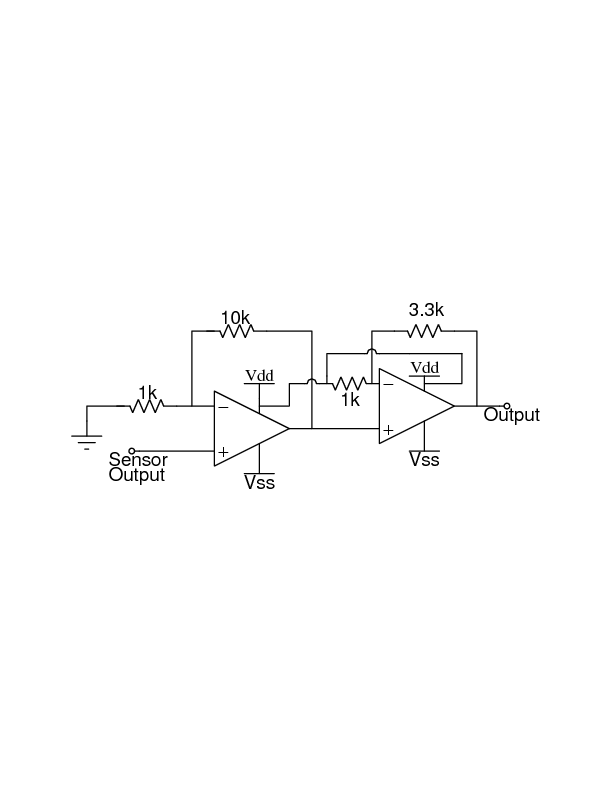
\includegraphics[width = 0.9\linewidth, trim = {0 10.25cm 0 10.5cm}, clip]{Hall_Effect_Sensor_Circuit.png}
	\caption{Hall Effect Sensor Circuit}
\end{figure}

\subsection{Part 2}

The circuit used in the first part was incorporated in this part in order to obtain the amplified and offset-removied output of the sensor when current was passed through the solenoid hence making it a temporary/electromagnetic magnet.\\
The current through the solenoid was controlled by varying voltage and a small resistance was connected in series to avoid a surge of current. An ammeter was also connected in series in order to measure the current through the solenoid. The output voltage of the sensor circuit was measured and plotted for varying current through the solenoid.

\begin{figure}[H]
	\centering
	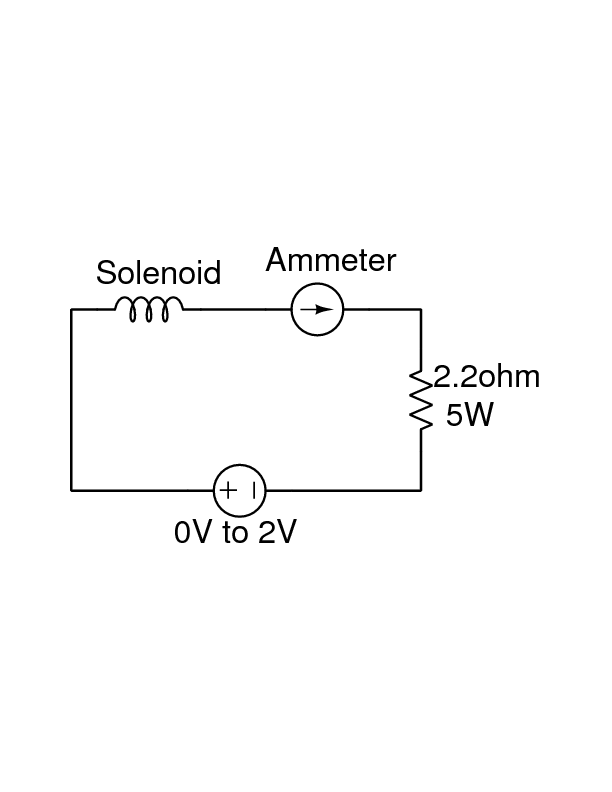
\includegraphics[width = 0.6\linewidth, trim = {0 8.5cm 0 8.5cm}, clip]{Solenoid_Circuit.png}
	\caption{Solenoid Circuit}
\end{figure}

\subsection{Part 3}

A DC motor was provided along with a circuit for an IR Pair sensor and connection points for the same. The apparatus also included a Hall-effect sensor whose output is digitised using a comparator - IC LM311. In this manner, the frequency of the outputs from the two sensor are compared. The Digital Storage Oscilloscope (DSO) was used for noting the square waves obtained from the comparator and the IR pair sensor. This process was repeated from several values of voltages across the DC motor; i.e. by varying the frequency of the DC motor.

\begin{figure}[H]
	\centering
	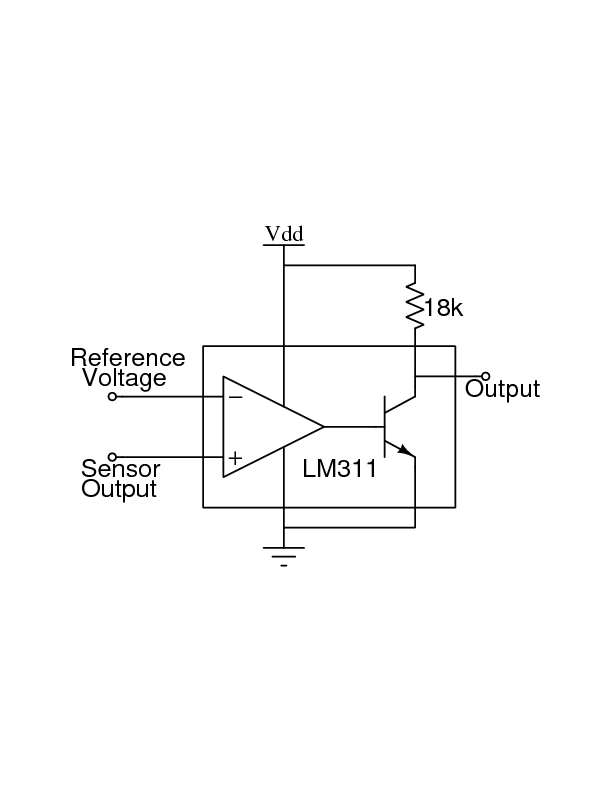
\includegraphics[width = 0.75\linewidth, trim = {0 7.5cm 0 7cm}, clip]{LM311_Comparator.png}
	\caption{LM311 Comparator}
\end{figure}

\section{Observations}

\subsection{Part 1}

The experiment was performed on a breadboard and measurement of the distance of the Neodymium magnet from the Hall-effect sensor was taken by a 15 cm ruler. Given below is a tabulation of the obtained output voltage for the corresponding distance of the magnet from the sensor.
\begin{table}[h!]
\centering
\begin{tabular}{||c|c||}
\hline\hline
Distance (cm) & Voltage (V)\\ [0.5ex]
\hline\hline
\(\infty\) & 0.00\\
15.0 & -0.01\\
11.0 & -0.04\\
8.7 & -0.07\\
7.5 & -0.12\\
6.5 & -0.17\\
5.8 & -0.24\\
5.3 & -0.30\\
4.7 & -0.41\\
4.3 & -0.51\\
4.0 & -0.63\\
3.7 & -0.82\\
3.3 & -1.09\\
3.0 & -1.35\\
2.7 & -1.71\\
2.3 & -2.35\\
2.0 & -3.05\\
1.7 & -1.44\\
1.3 & -6.61\\
1.0 & -11.05\\
0.7 & -11.97\\ [1ex]
\hline\hline
\end{tabular}
\end{table}

\begin{figure}[H]
	\centering
	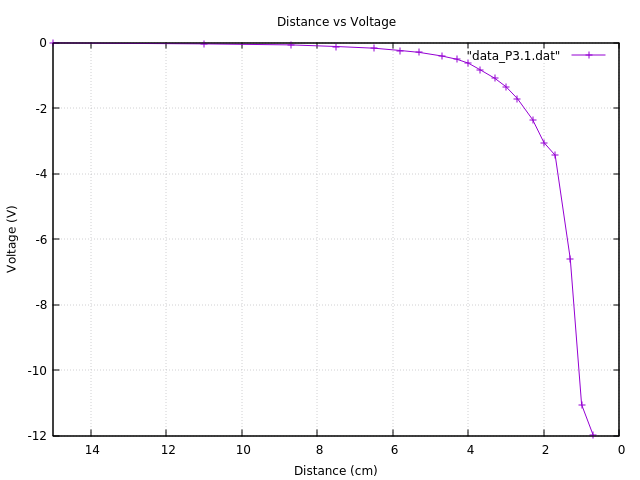
\includegraphics[width = 0.75\linewidth, trim = {0 0 0 0}, clip]{Part 1 - Distance vs Voltage.png}
	\caption{Distance vs Voltage}
\end{figure}

From this plot, we can quite clearly see that, as distance decreases, the output voltage increases, which further implies that the magnetic flux passing through a given area is inversely proportional to the distance of the source of the magnetic flux from that area.\\
Also, on changing the polarity of the magnet, there is no significant change since the magnetic flux will simply be the negative on what the original case had shown.

\subsection{Part 2}

The experiment was again performed primarily on the breadboard. The solenoid was placed perpendicular to the breadboard at a constant distance. Given below is a tabulation of the obtained output voltage for the corresponding current passing through the solenoid, hence making it function by the formula:
\[ \Phi_{SOL} \propto B\cdot A \propto \mu nI \] where \( \Phi_{SOL} \) represents the magnetic flux through the sensor, B represents the magnetic field, A represents the sensing area, \( \mu \) represents the magnetic permeability, n represents the number of turns and I represents the current flowing through the solenoid.\\
The first section of the table differs from the second in the fact that the current had been reversed for measuring the voltages for the second section.
\begin{table}[h!]
\centering
\begin{tabular}{||c|c||c|c||}
\hline\hline
Normal current(mA) & Voltage(V) & Reversed Current(mA) & Voltage(V)\\ [0.5ex]
\hline\hline
6 & 0.35 & -11 & 0.25 \\
43 & 0.82 & -40 & 0.53 \\
94 & 1.78 & -72 & 1.59 \\
141 & 2.59 & -129 & 2.53 \\
192 & 3.42 & -183 & 3.38 \\
240 & 4.15 & -225 & 4.14 \\
292 & 4.88 & -285 & 4.75 \\
345 & 5.57 & -337 & 5.58 \\
400 & 6.39 & -398 & 6.42 \\
438 & 6.59 & -420 & 6.45 \\
490 & 6.91 & -469 & 6.89 \\ [1ex]
\hline\hline
\end{tabular}
\end{table}

\begin{figure}[H]
	\begin{subfigure}[b]{0.5\linewidth}
		\centering
		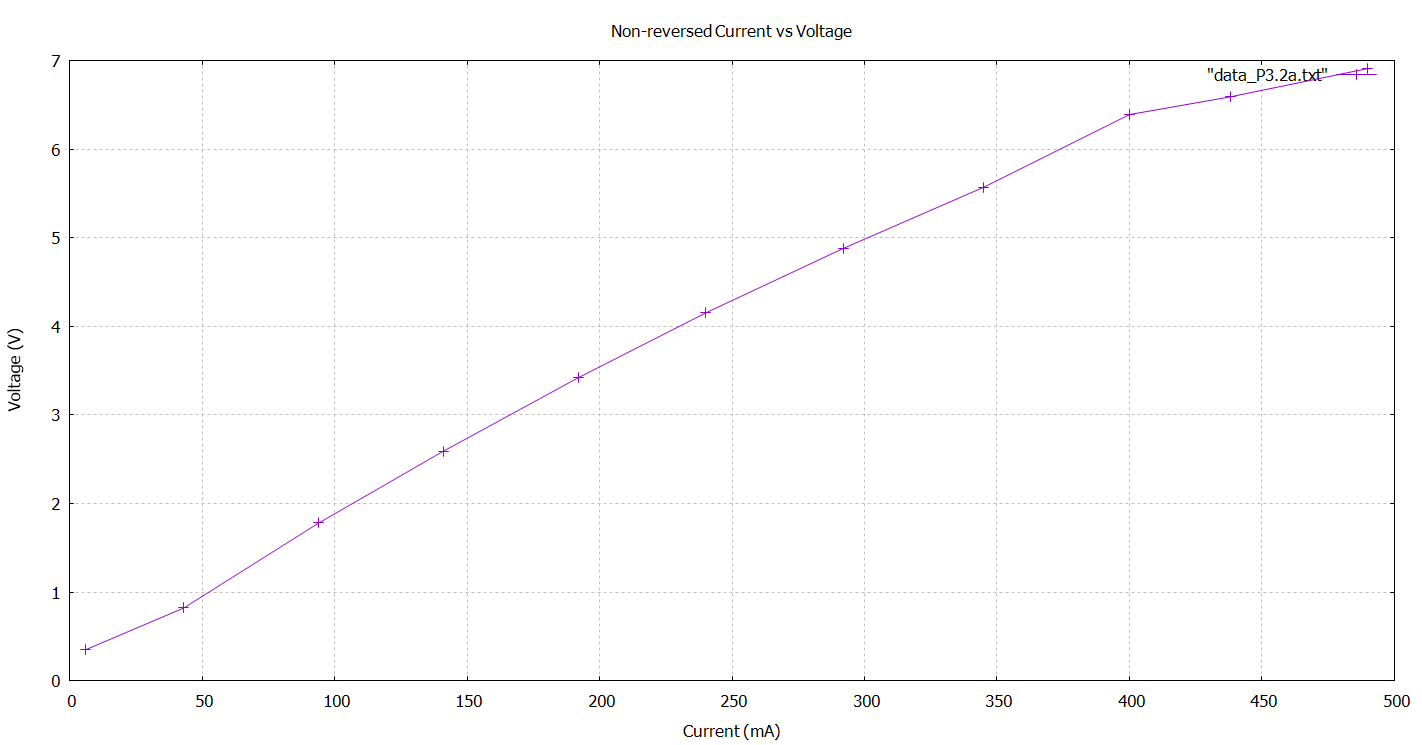
\includegraphics[width = 0.85\linewidth, trim = {0 0 0 0}, clip]{Part_2_Irreversed_Current_vs_Voltage.png}
		\caption{With non-reversed Current}
	\end{subfigure}
	\begin{subfigure}[b]{0.5\linewidth}
		\centering
		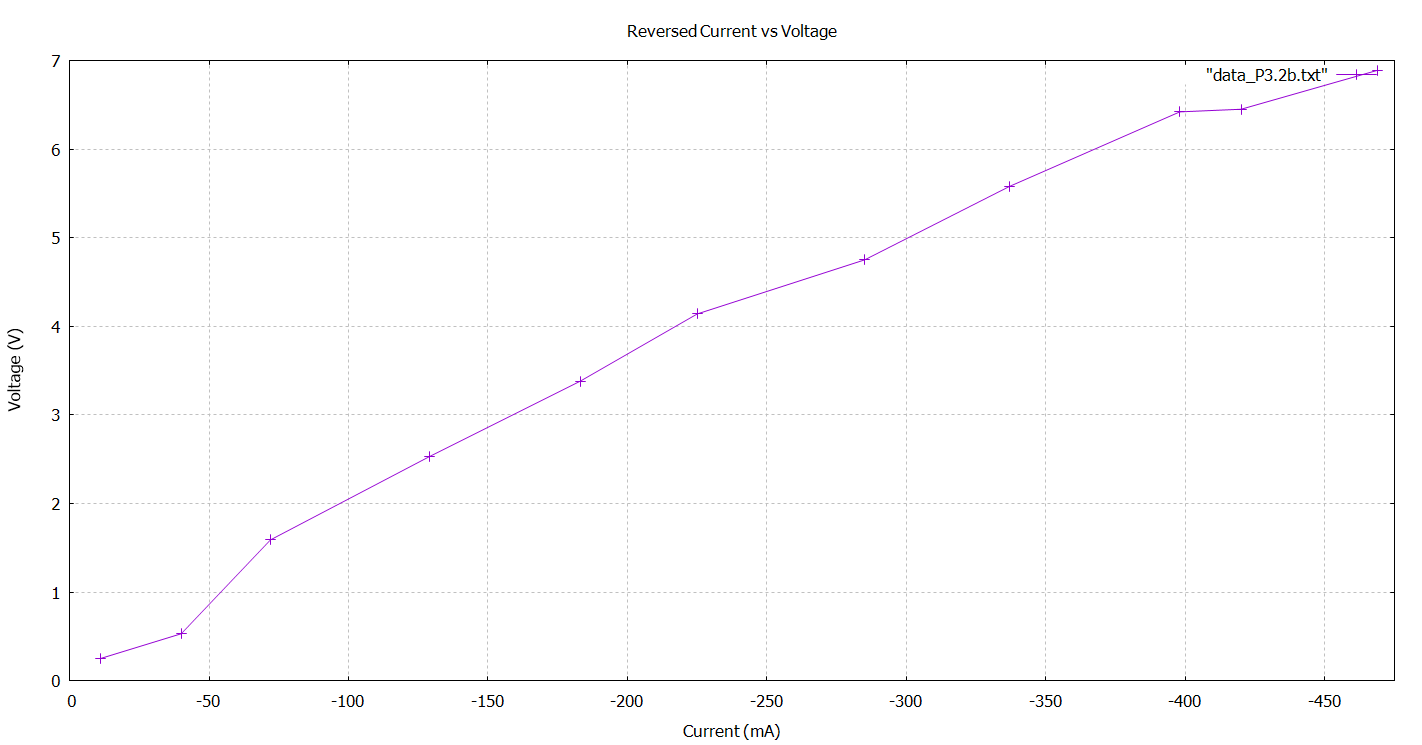
\includegraphics[width = 0.85\linewidth, trim = {0 0 0 0}, clip]{Part_2_Reversed_Current_vs_Voltage.png}
		\caption{With reversed Current}
	\end{subfigure}
		\caption{Current vs Voltage}
\end{figure}

As is clearly observable seen, the output voltage is directly proportional to the current passed through the solenoid and the dependence on the direction of current is meagre.

\subsection{Part 3}

The experiment was primarily performed on the DC motor assembly with the breadboard as a complimentary piece on which the comparator circuit was built. Given below is the tabulation of the voltage applied on the DC motor (\( V_{MOTOR} \)) with the frequency of output of the Hall-effect sensor (\( \nu_{HES} \)) , the frequency of output of the IR pair sensor (\( \nu_{IR} \)) and the ratio \( \frac{\nu_{IR}}{\nu_{HES}} \).
\begin{table}[h!]
\centering
\begin{tabular}{||c||c|c|c||}
\hline\hline
\( V_{MOTOR} \)(V) & \( \nu_{HES} \)(Hz) & \( \nu_{IR} \)(Hz) & \( \frac{\nu_{IR}}{\nu_{HES}} \)\\ [0.5ex]
\hline\hline
3.0 & 1.748 & 50.00 & 28.60\\
4.0 & 2.404 & 71.43 & 29.71\\
4.5 & 2.747 & 83.33 & 30.34\\
6.6 & 4.149 & 125.00 & 30.13\\
9.0 & 5.714 & 166.70 & 29.17\\ [1ex]
\hline\hline
\end{tabular}
\end{table}

On the average, the ratio is 29.59 which can be approximated to 30.\\

\begin{figure}[H]
	\begin{subfigure}[b]{0.5\linewidth}		
		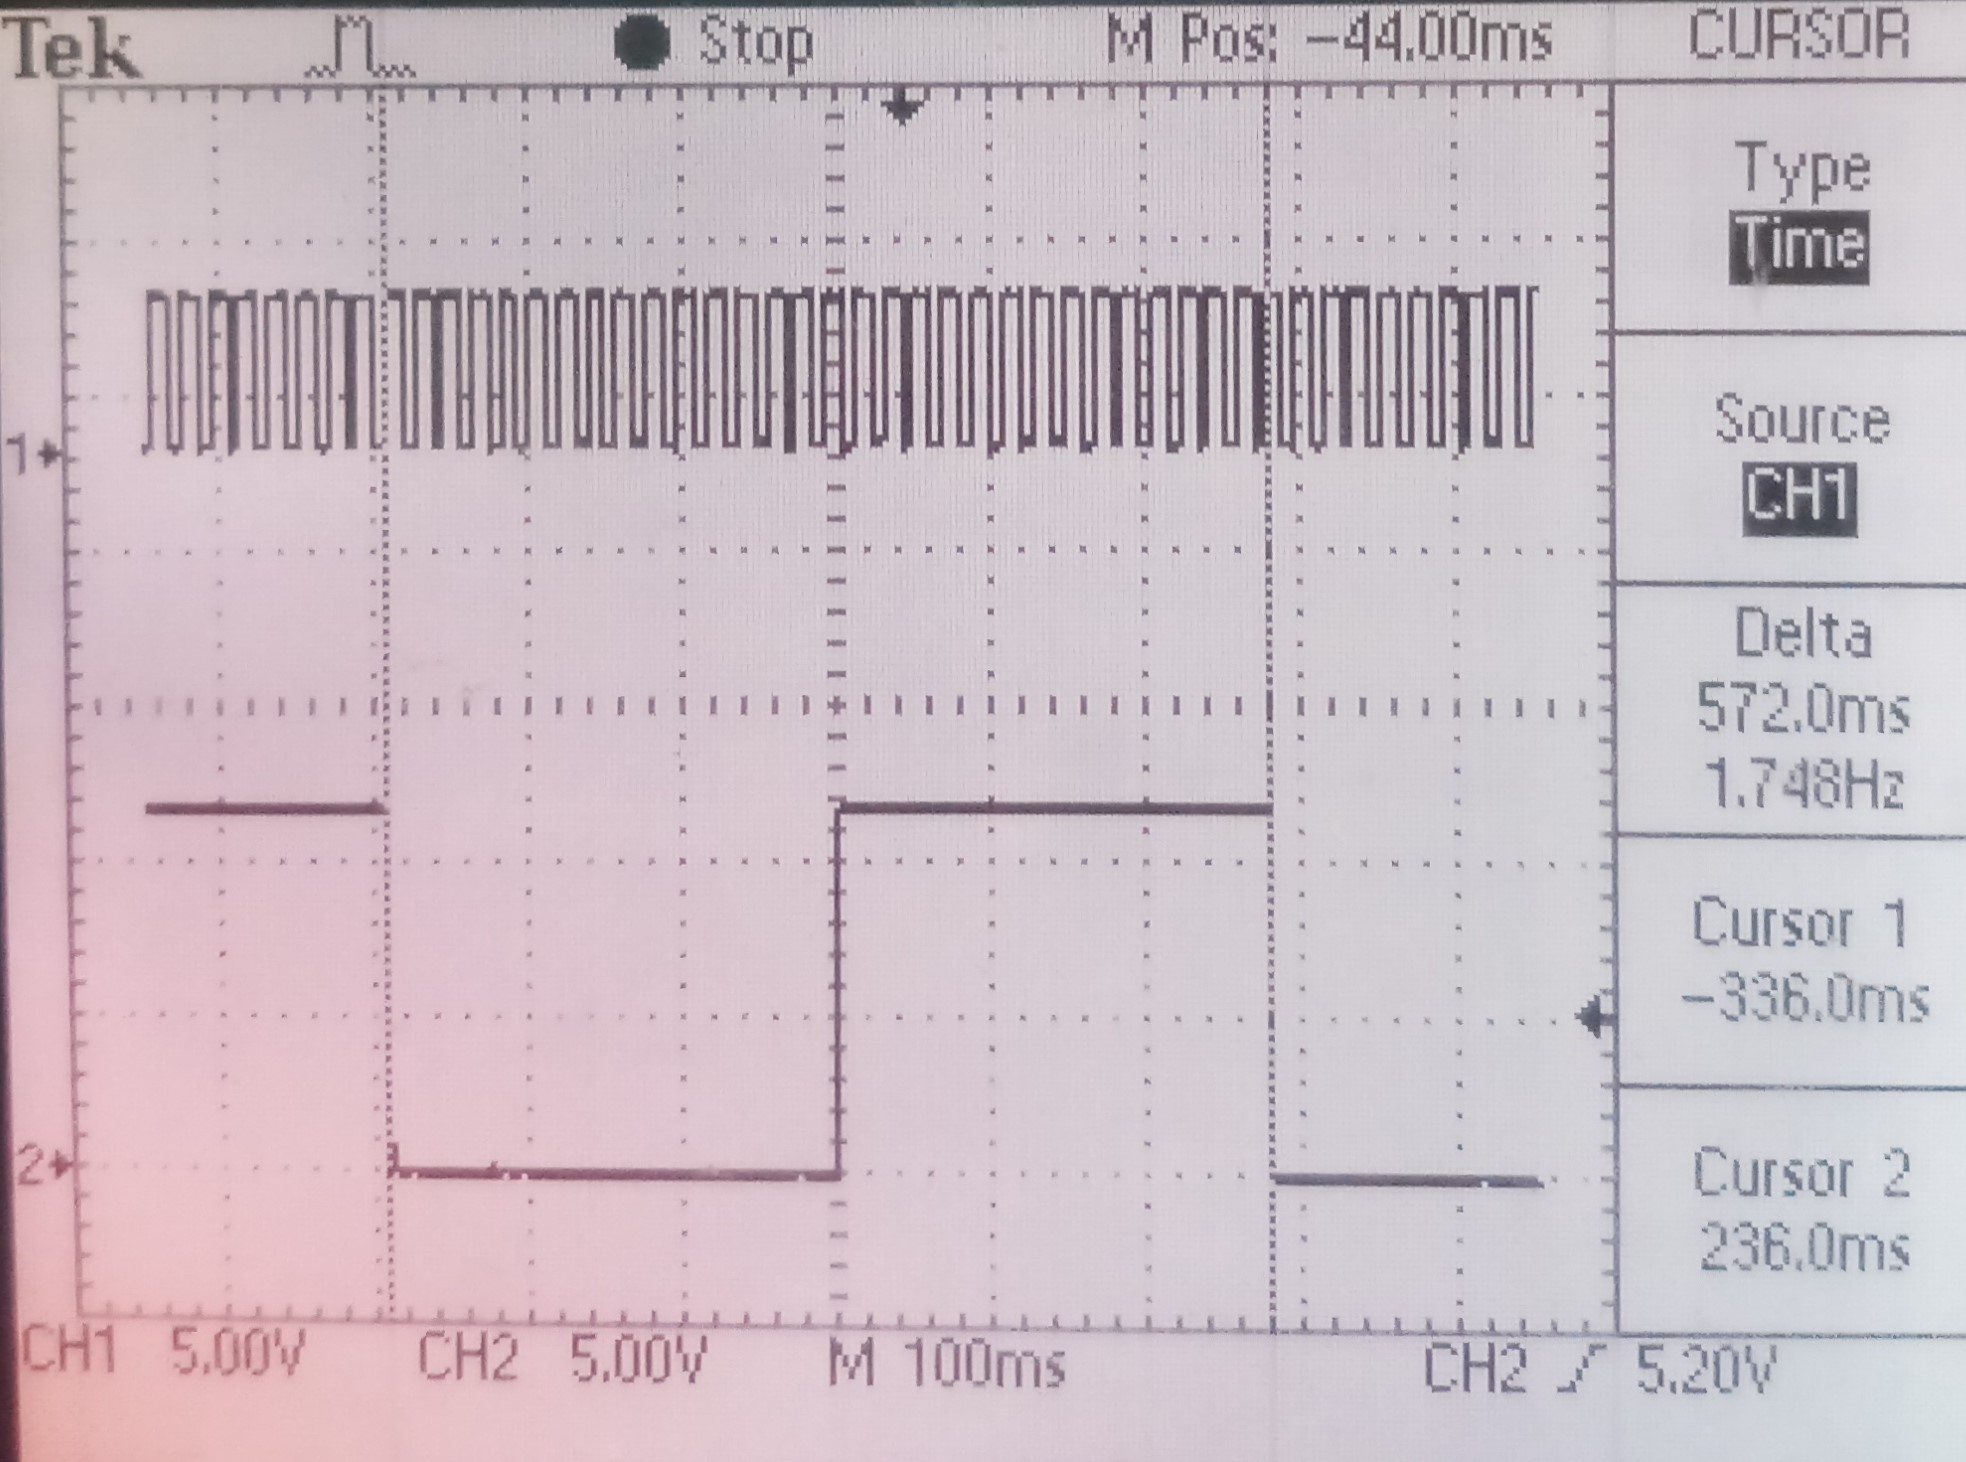
\includegraphics[width = \linewidth, trim = {0 0 0 0}, clip]{HES3V.jpg}
		\caption{\( \nu_{HES} \)}
	\end{subfigure}
	\begin{subfigure}[b]{0.5\linewidth}						
		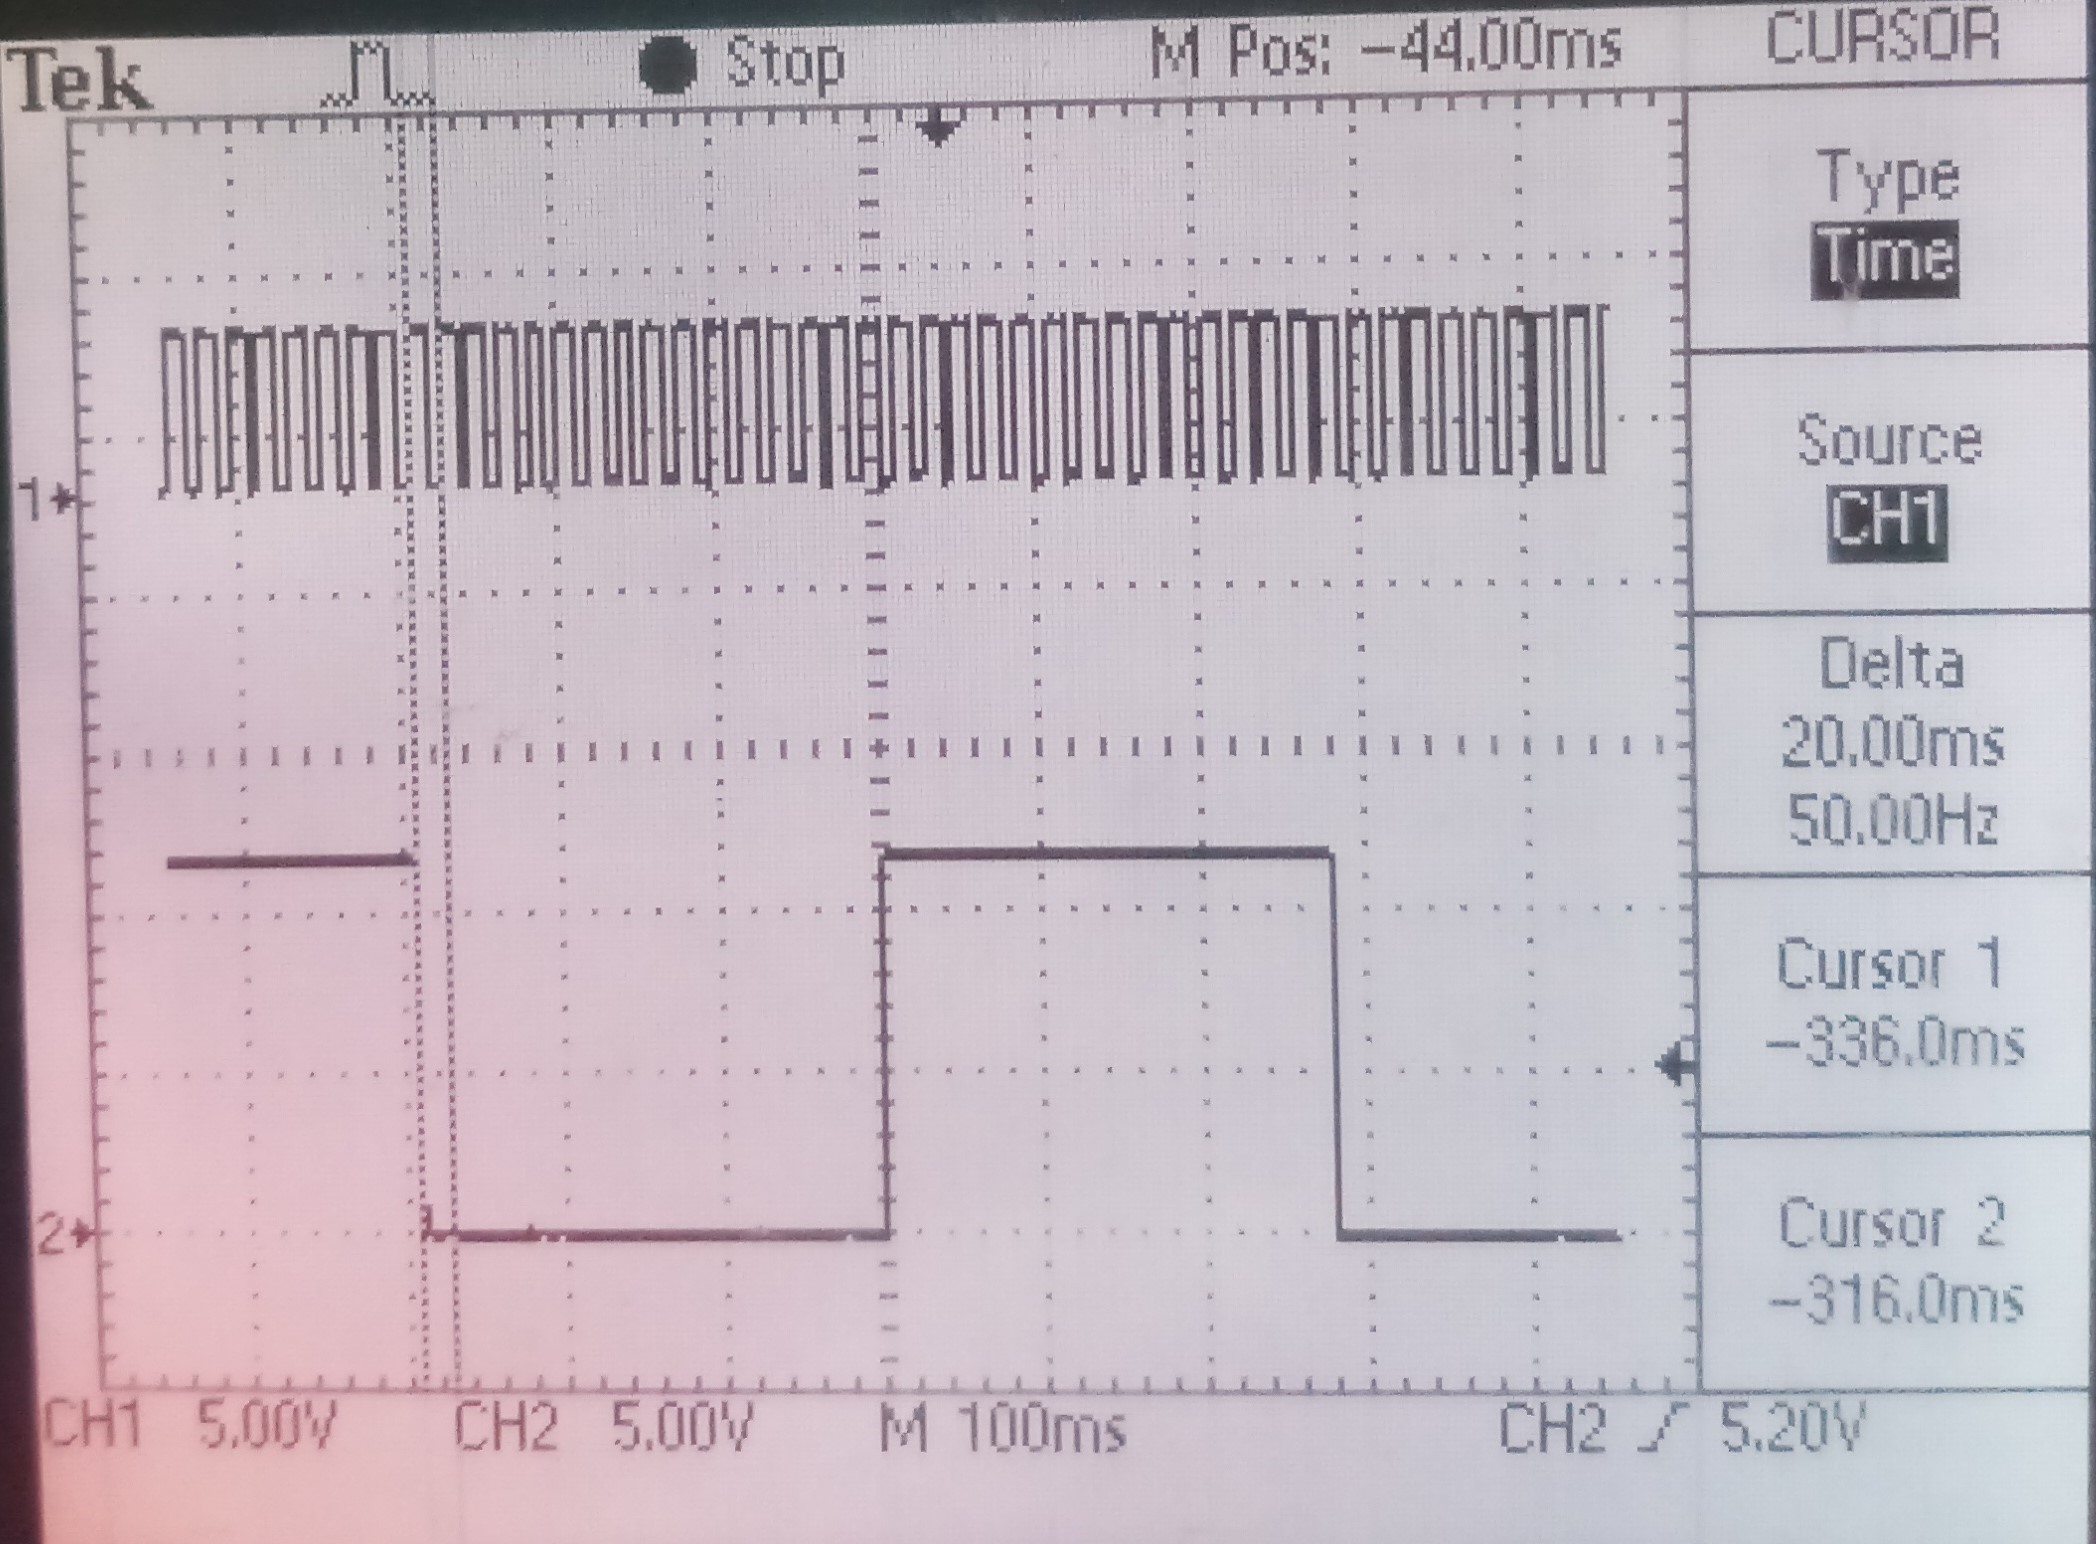
\includegraphics[width = \linewidth, trim = {0 0 0 0}, clip]{IR3V.jpg}
		\caption{\( \nu_{IR} \)}
	\end{subfigure}
	\caption{Oscillator snapshots for 3V}
\end{figure}
\begin{figure}[H]
	\begin{subfigure}[b]{0.5\linewidth}		
		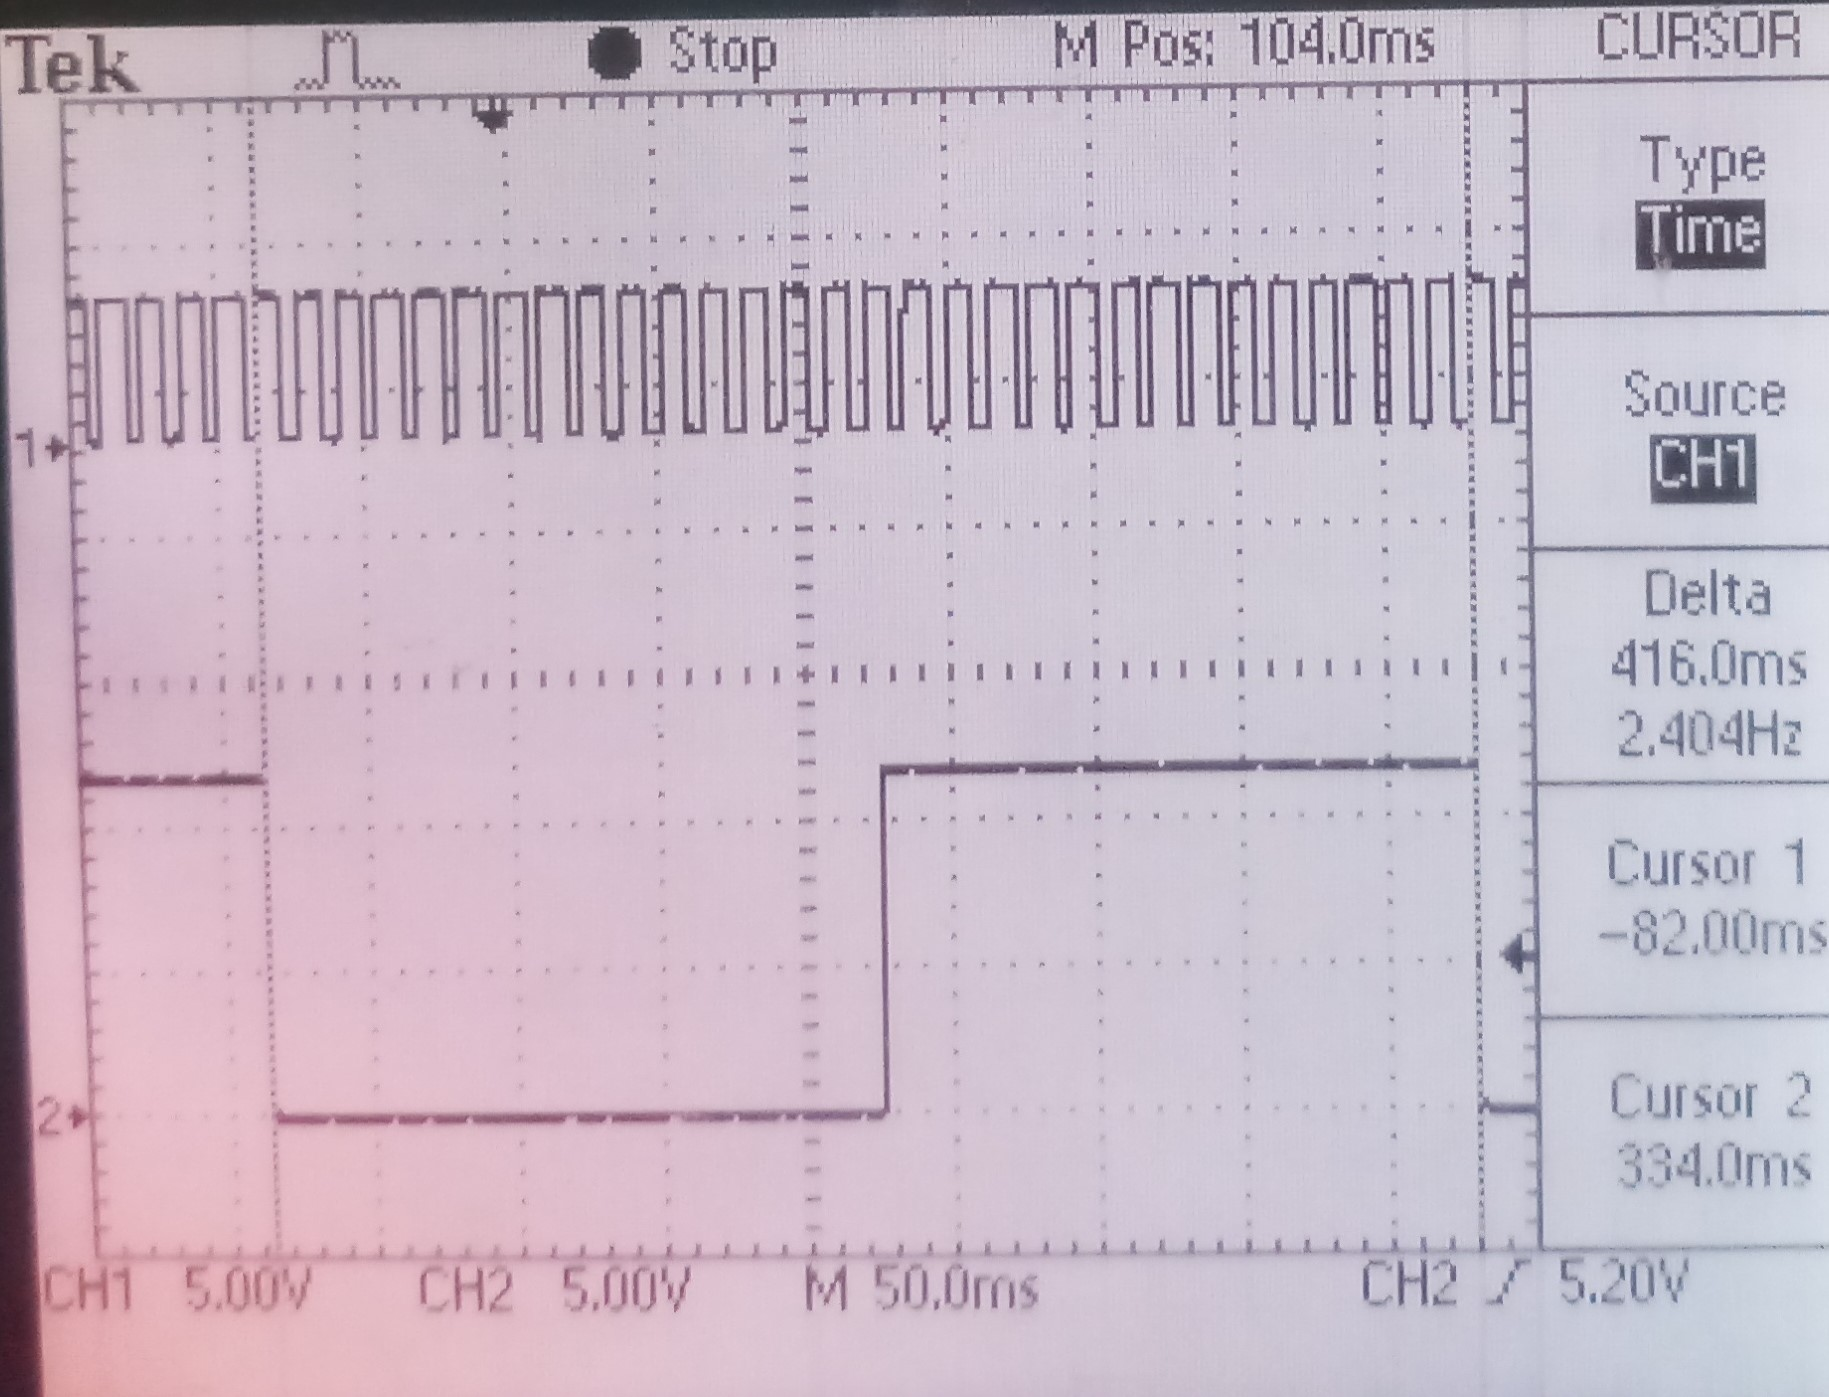
\includegraphics[width = \linewidth, trim = {0 0 0 0}, clip]{HES4V.jpg}
		\caption{\( \nu_{HES} \)}
	\end{subfigure}
	\begin{subfigure}[b]{0.5\linewidth}						
		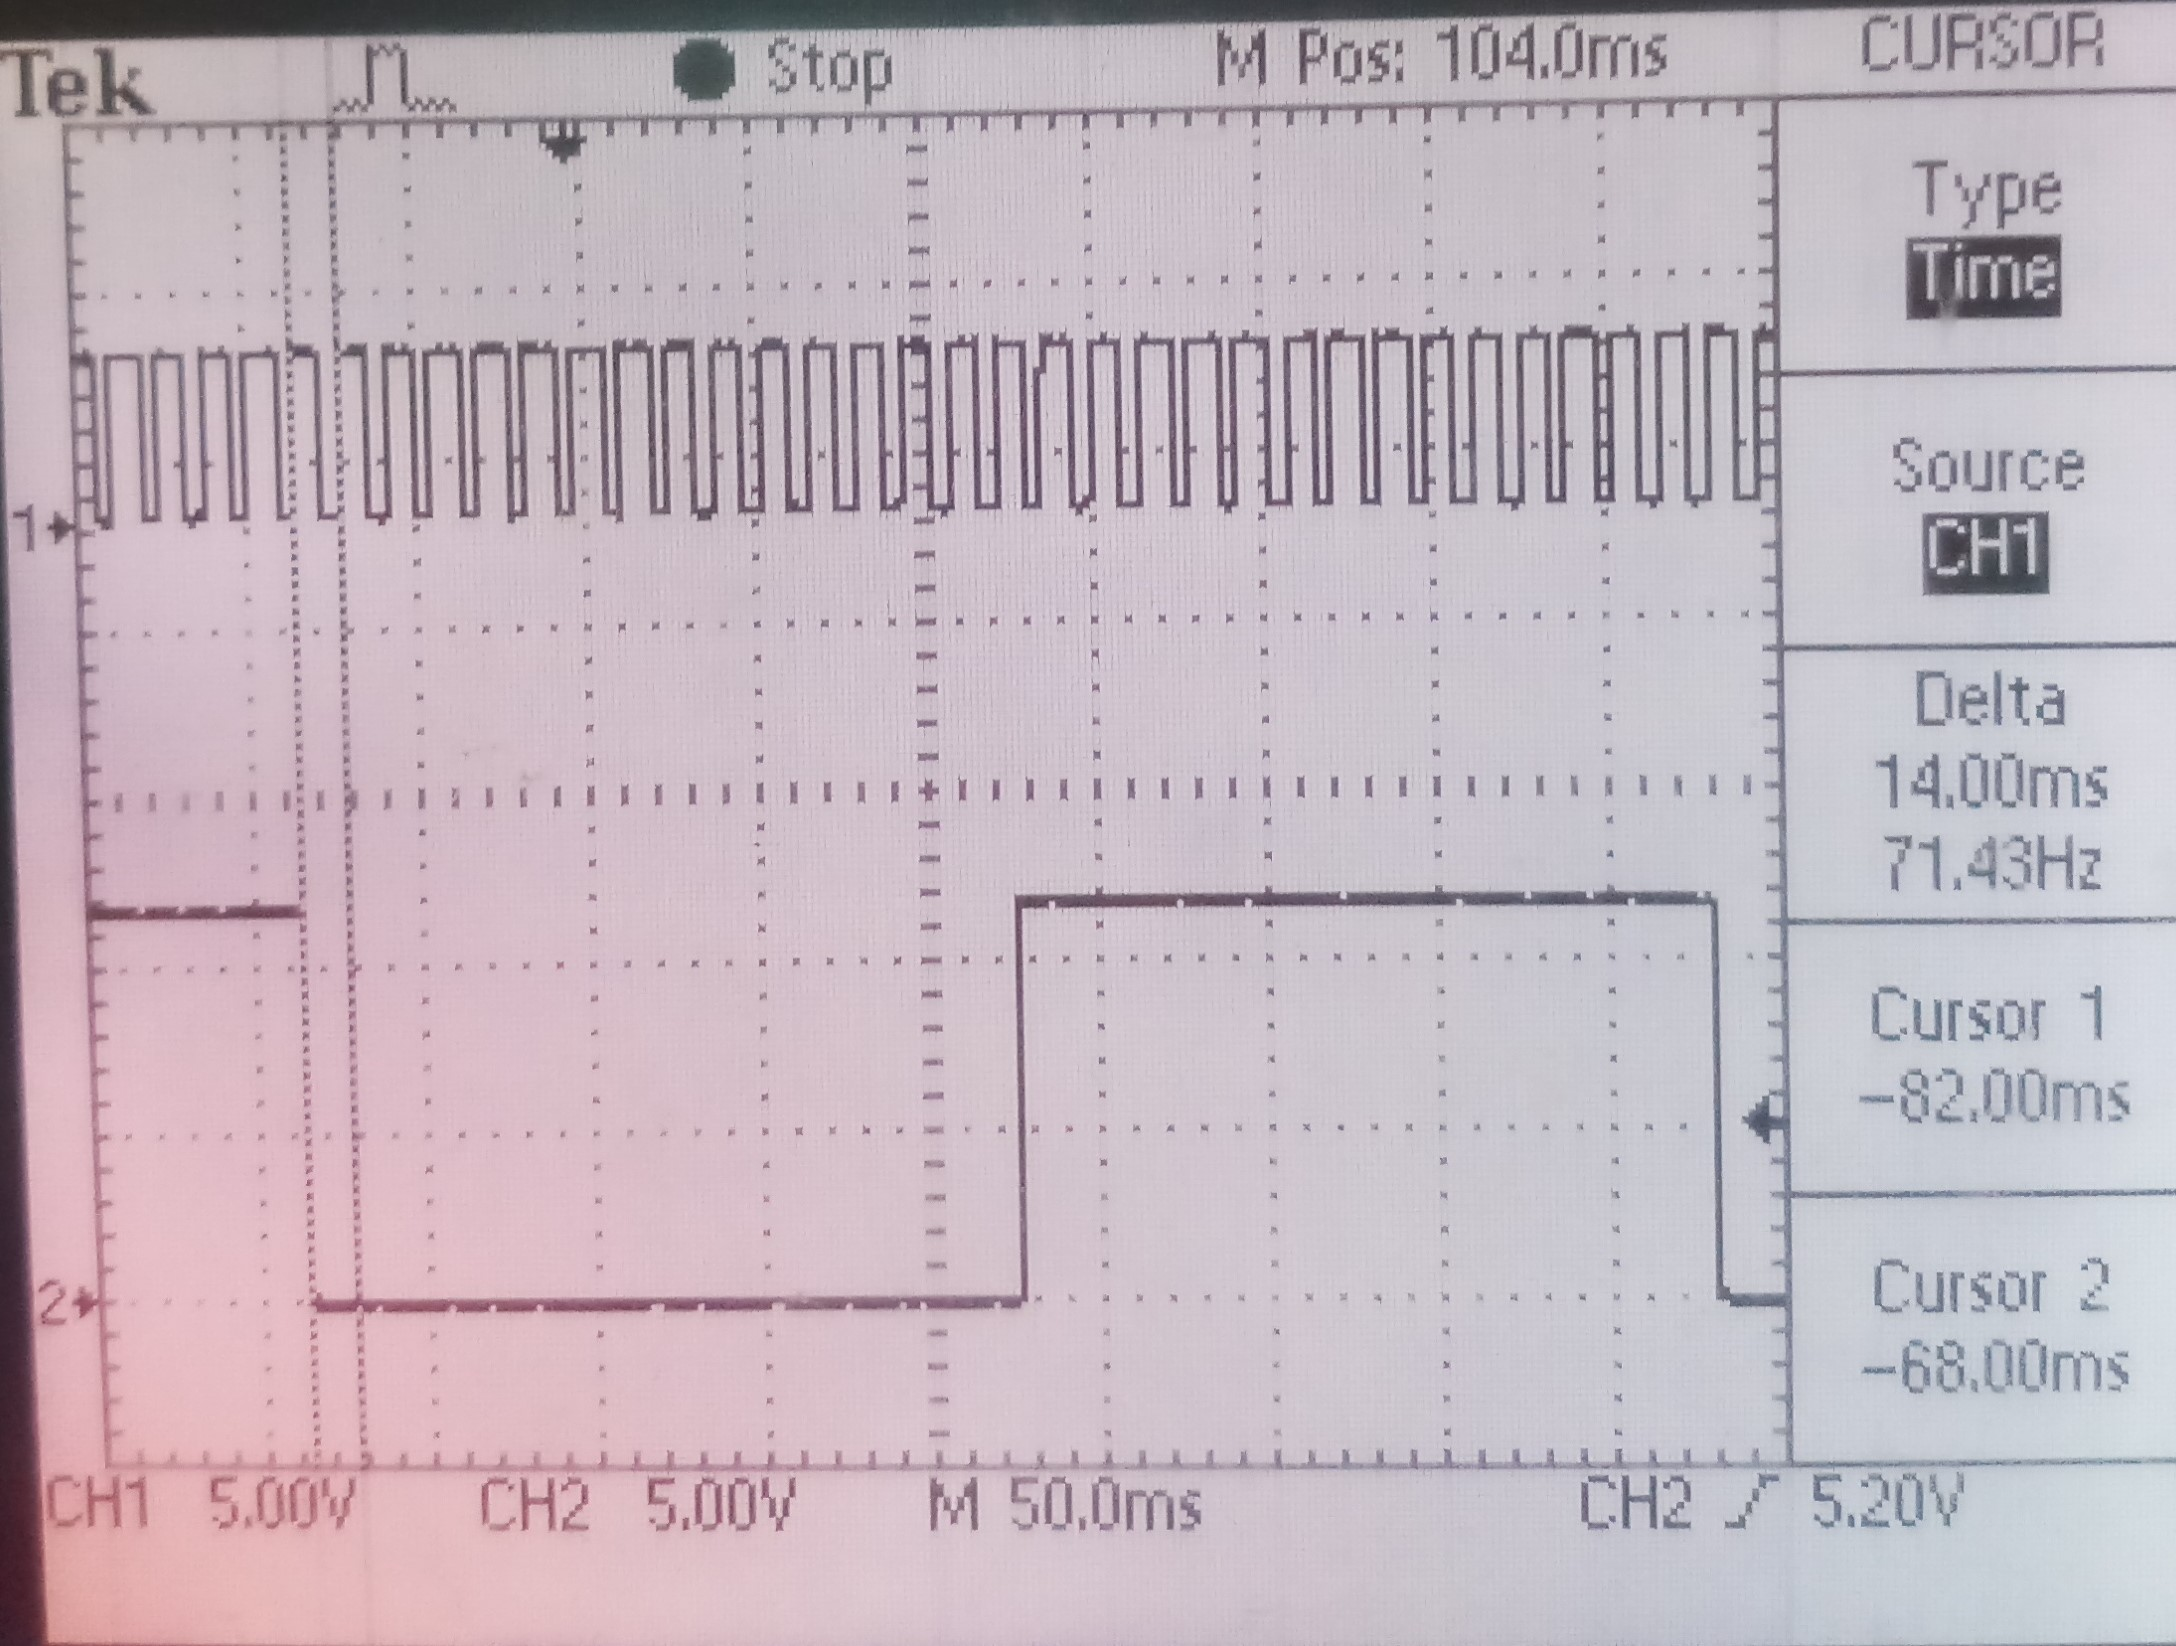
\includegraphics[width = \linewidth, trim = {0 0 0 0}, clip]{IR4V.jpg}
		\caption{\( \nu_{IR} \)}
	\end{subfigure}
	\caption{Oscillator snapshots for 4V}
\end{figure}
\begin{figure}[H]
	\begin{subfigure}[b]{0.5\linewidth}
		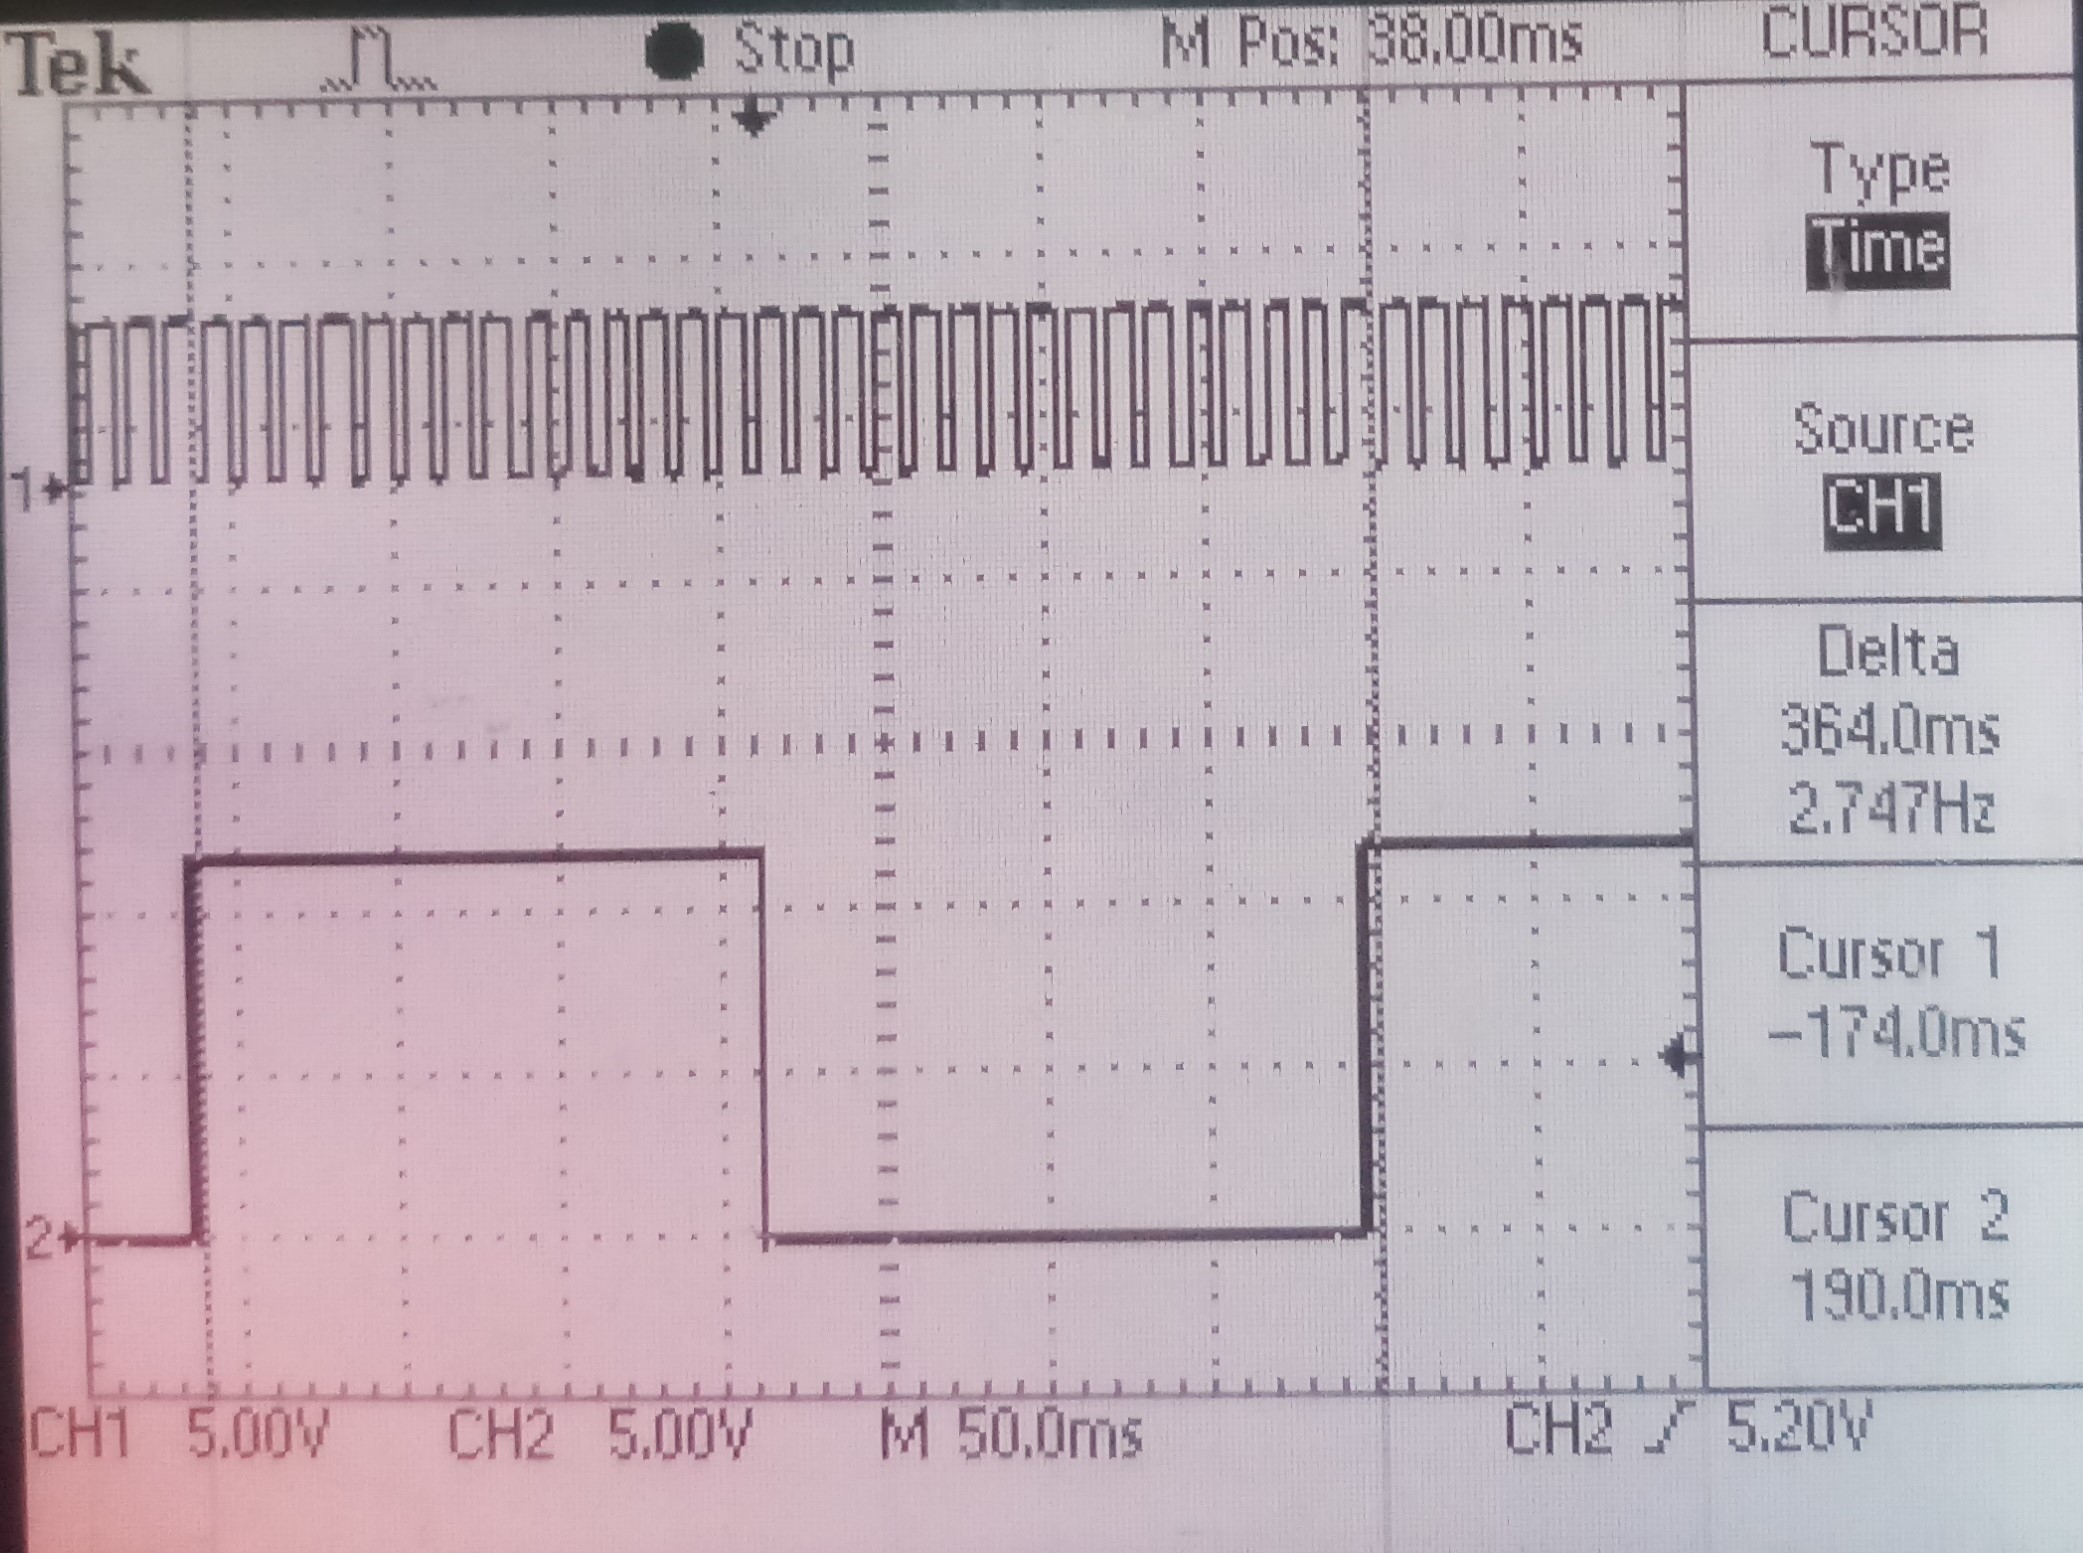
\includegraphics[width = \linewidth, trim = {0 0 0 0}, clip]{HES4_5V.jpg}
		\caption{\( \nu_{HES} \)}
	\end{subfigure}
	\begin{subfigure}[b]{0.5\linewidth}						
		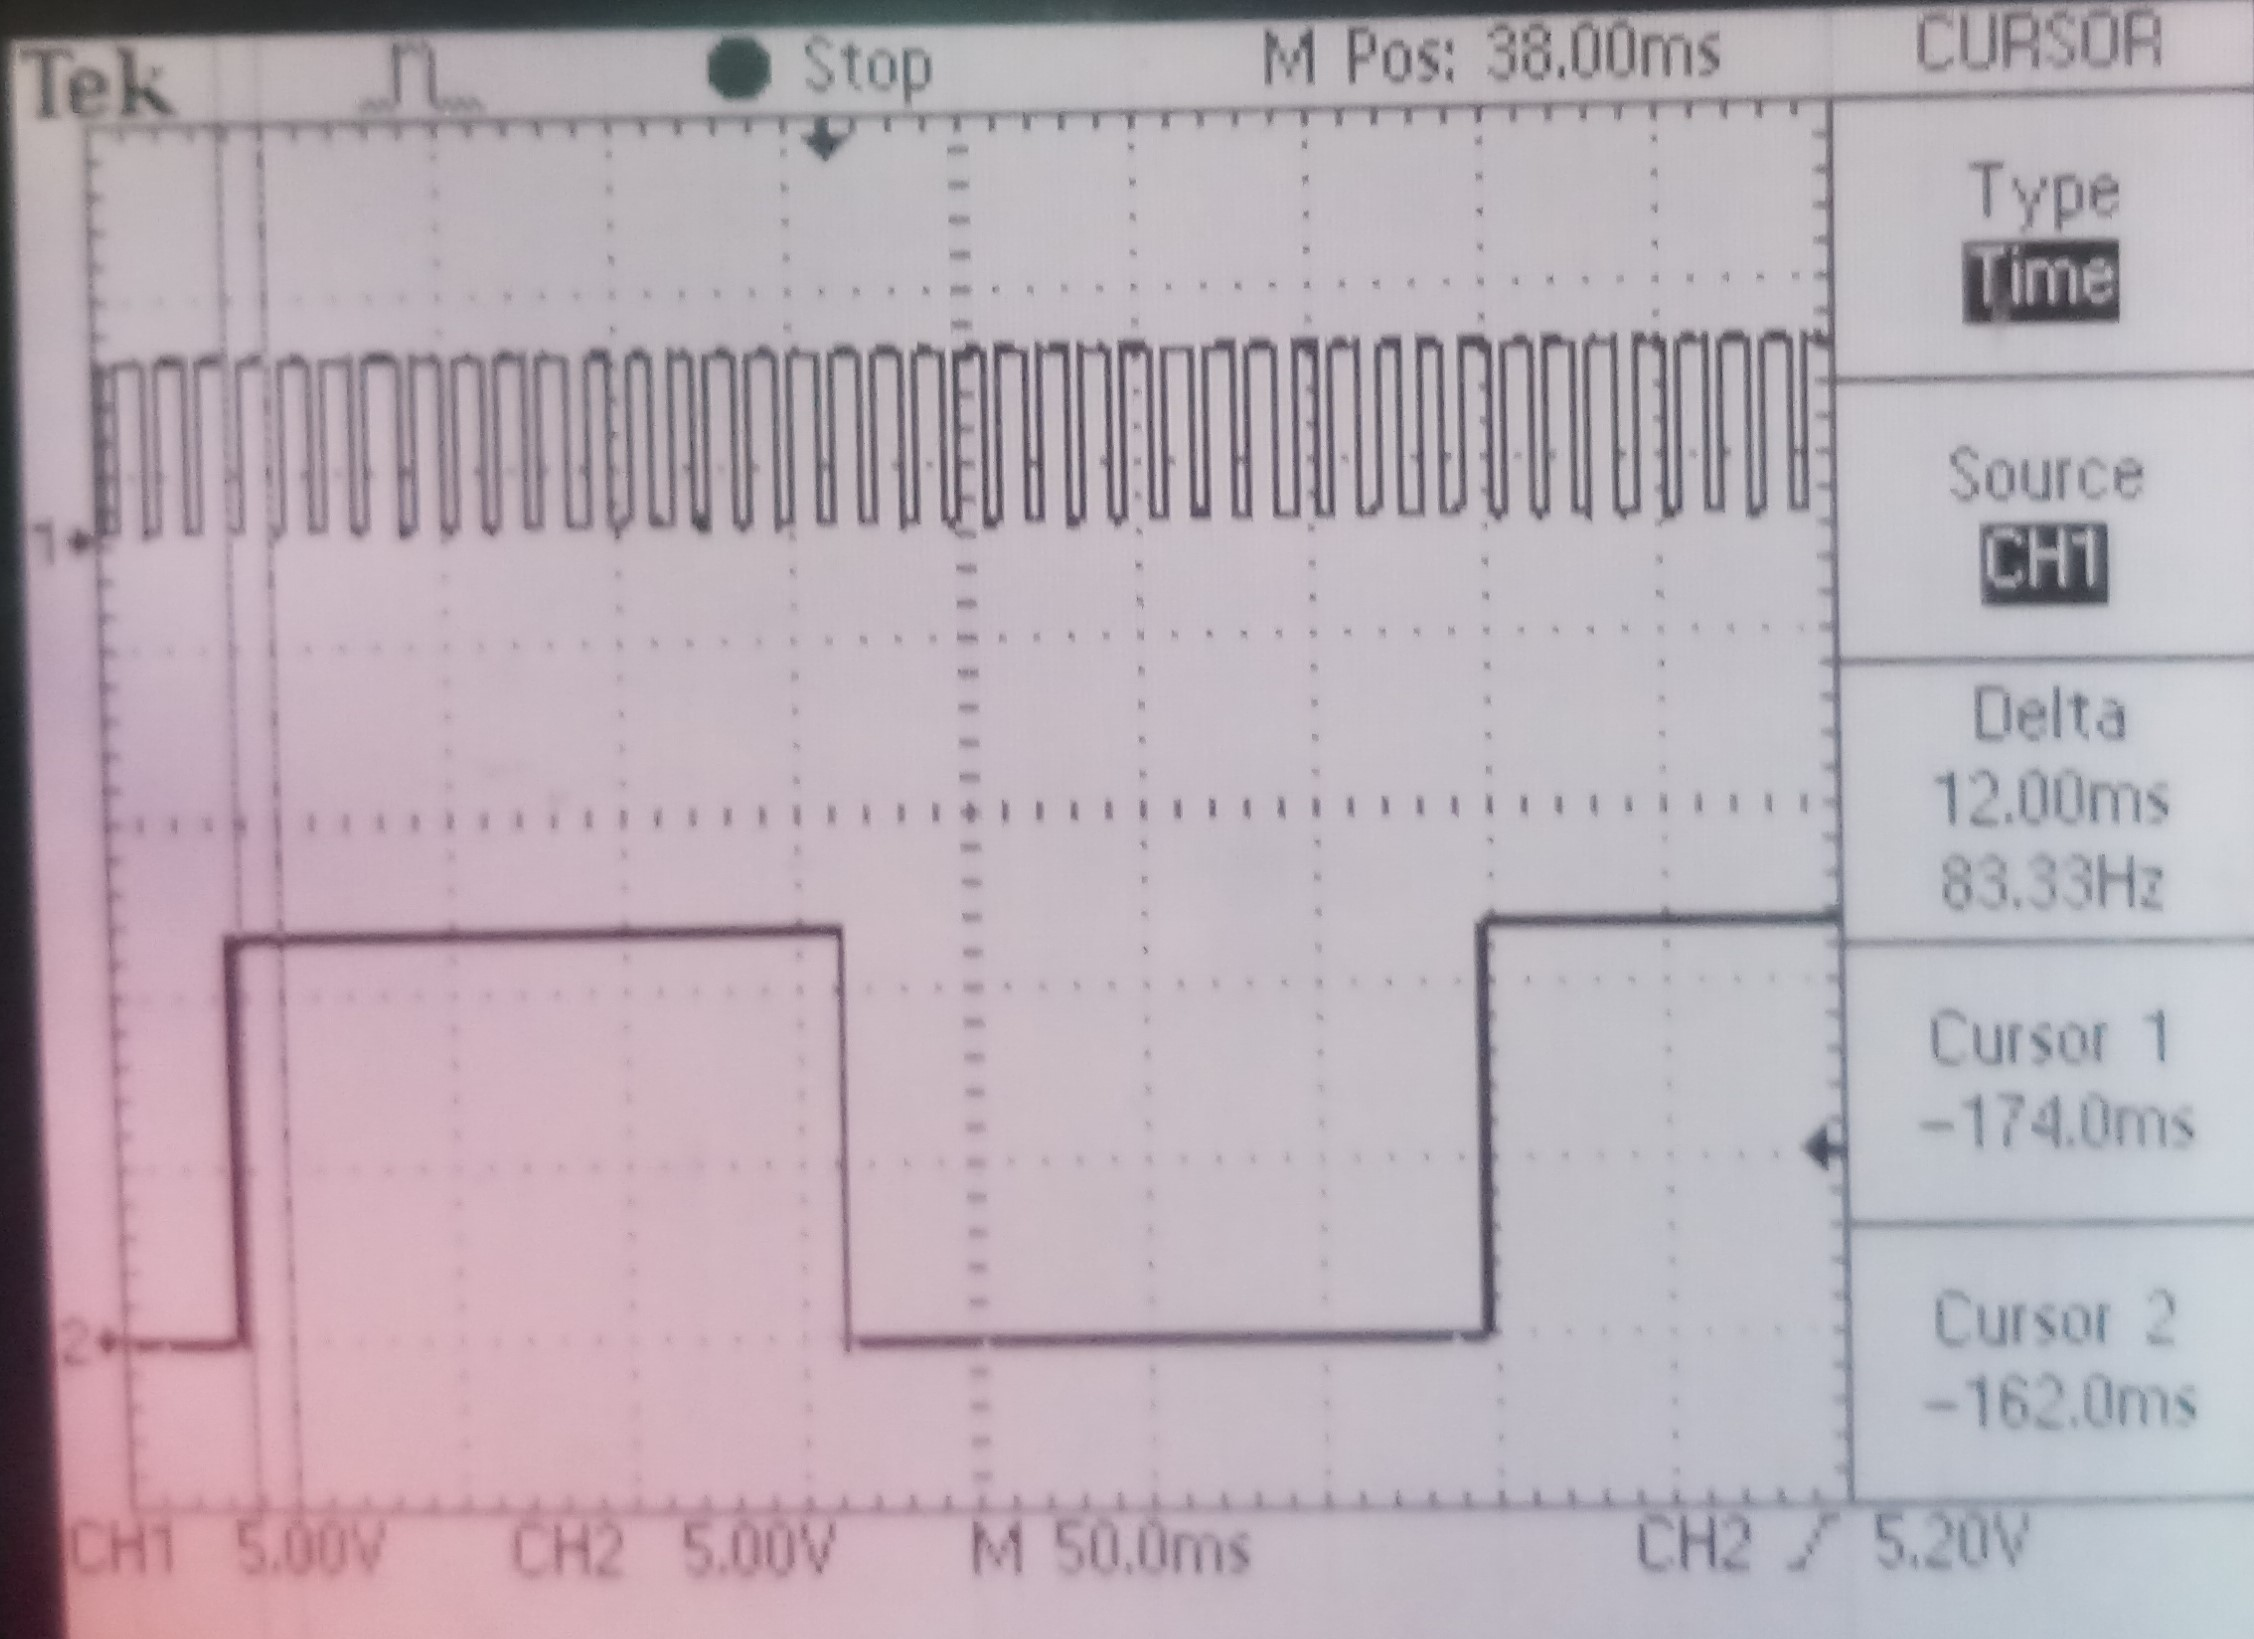
\includegraphics[width = \linewidth, trim = {0 0 0 0}, clip]{IR4_5V.jpg}
		\caption{\( \nu_{IR} \)}
	\end{subfigure}
	\caption{Oscillator snapshots for 4.5V}
\end{figure}
\begin{figure}[H]
	\begin{subfigure}[b]{0.5\linewidth}		
		\includegraphics[width = \linewidth, trim = {0 0 0 0}, clip]{HES6_6V.jpg}
		\caption{\( \nu_{HES} \)}
	\end{subfigure}
	\begin{subfigure}[b]{0.5\linewidth}						
		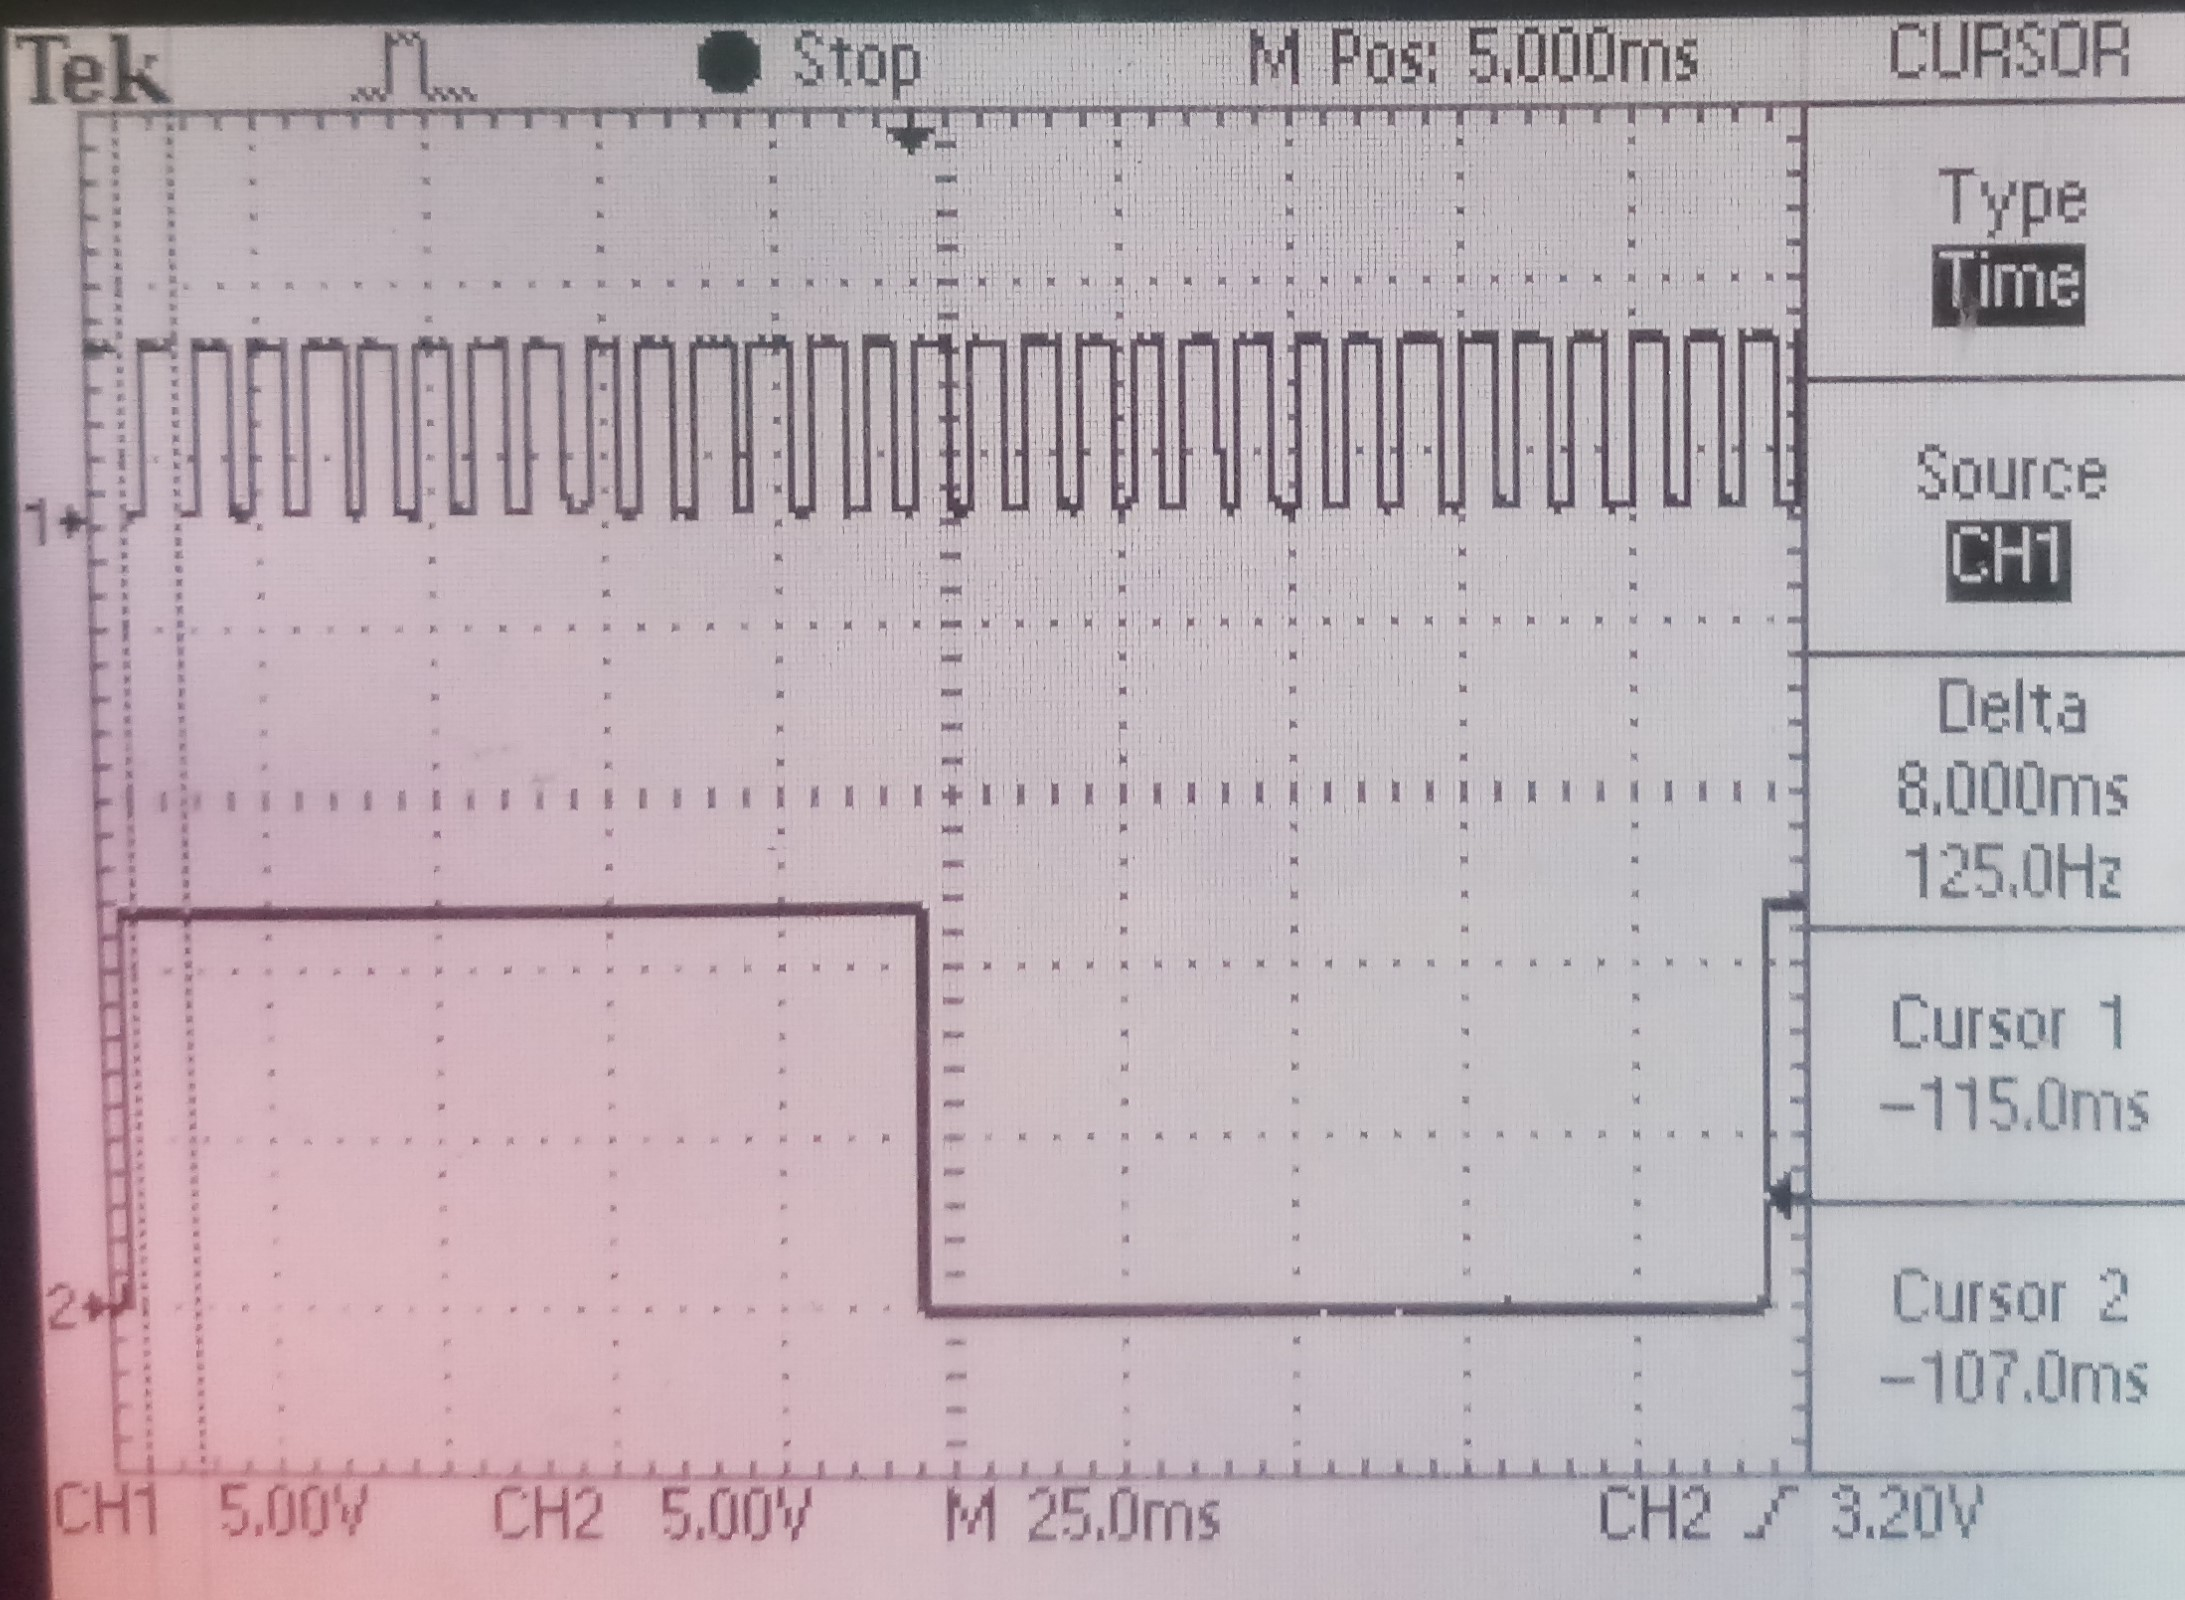
\includegraphics[width = \linewidth, trim = {0 0 0 0}, clip]{IR6_6V.jpg}
		\caption{\( \nu_{IR} \)}
	\end{subfigure}
	\caption{Oscillator snapshots for 6.6V}
\end{figure}
\begin{figure}[H]
	\begin{subfigure}[b]{0.5\linewidth}		
		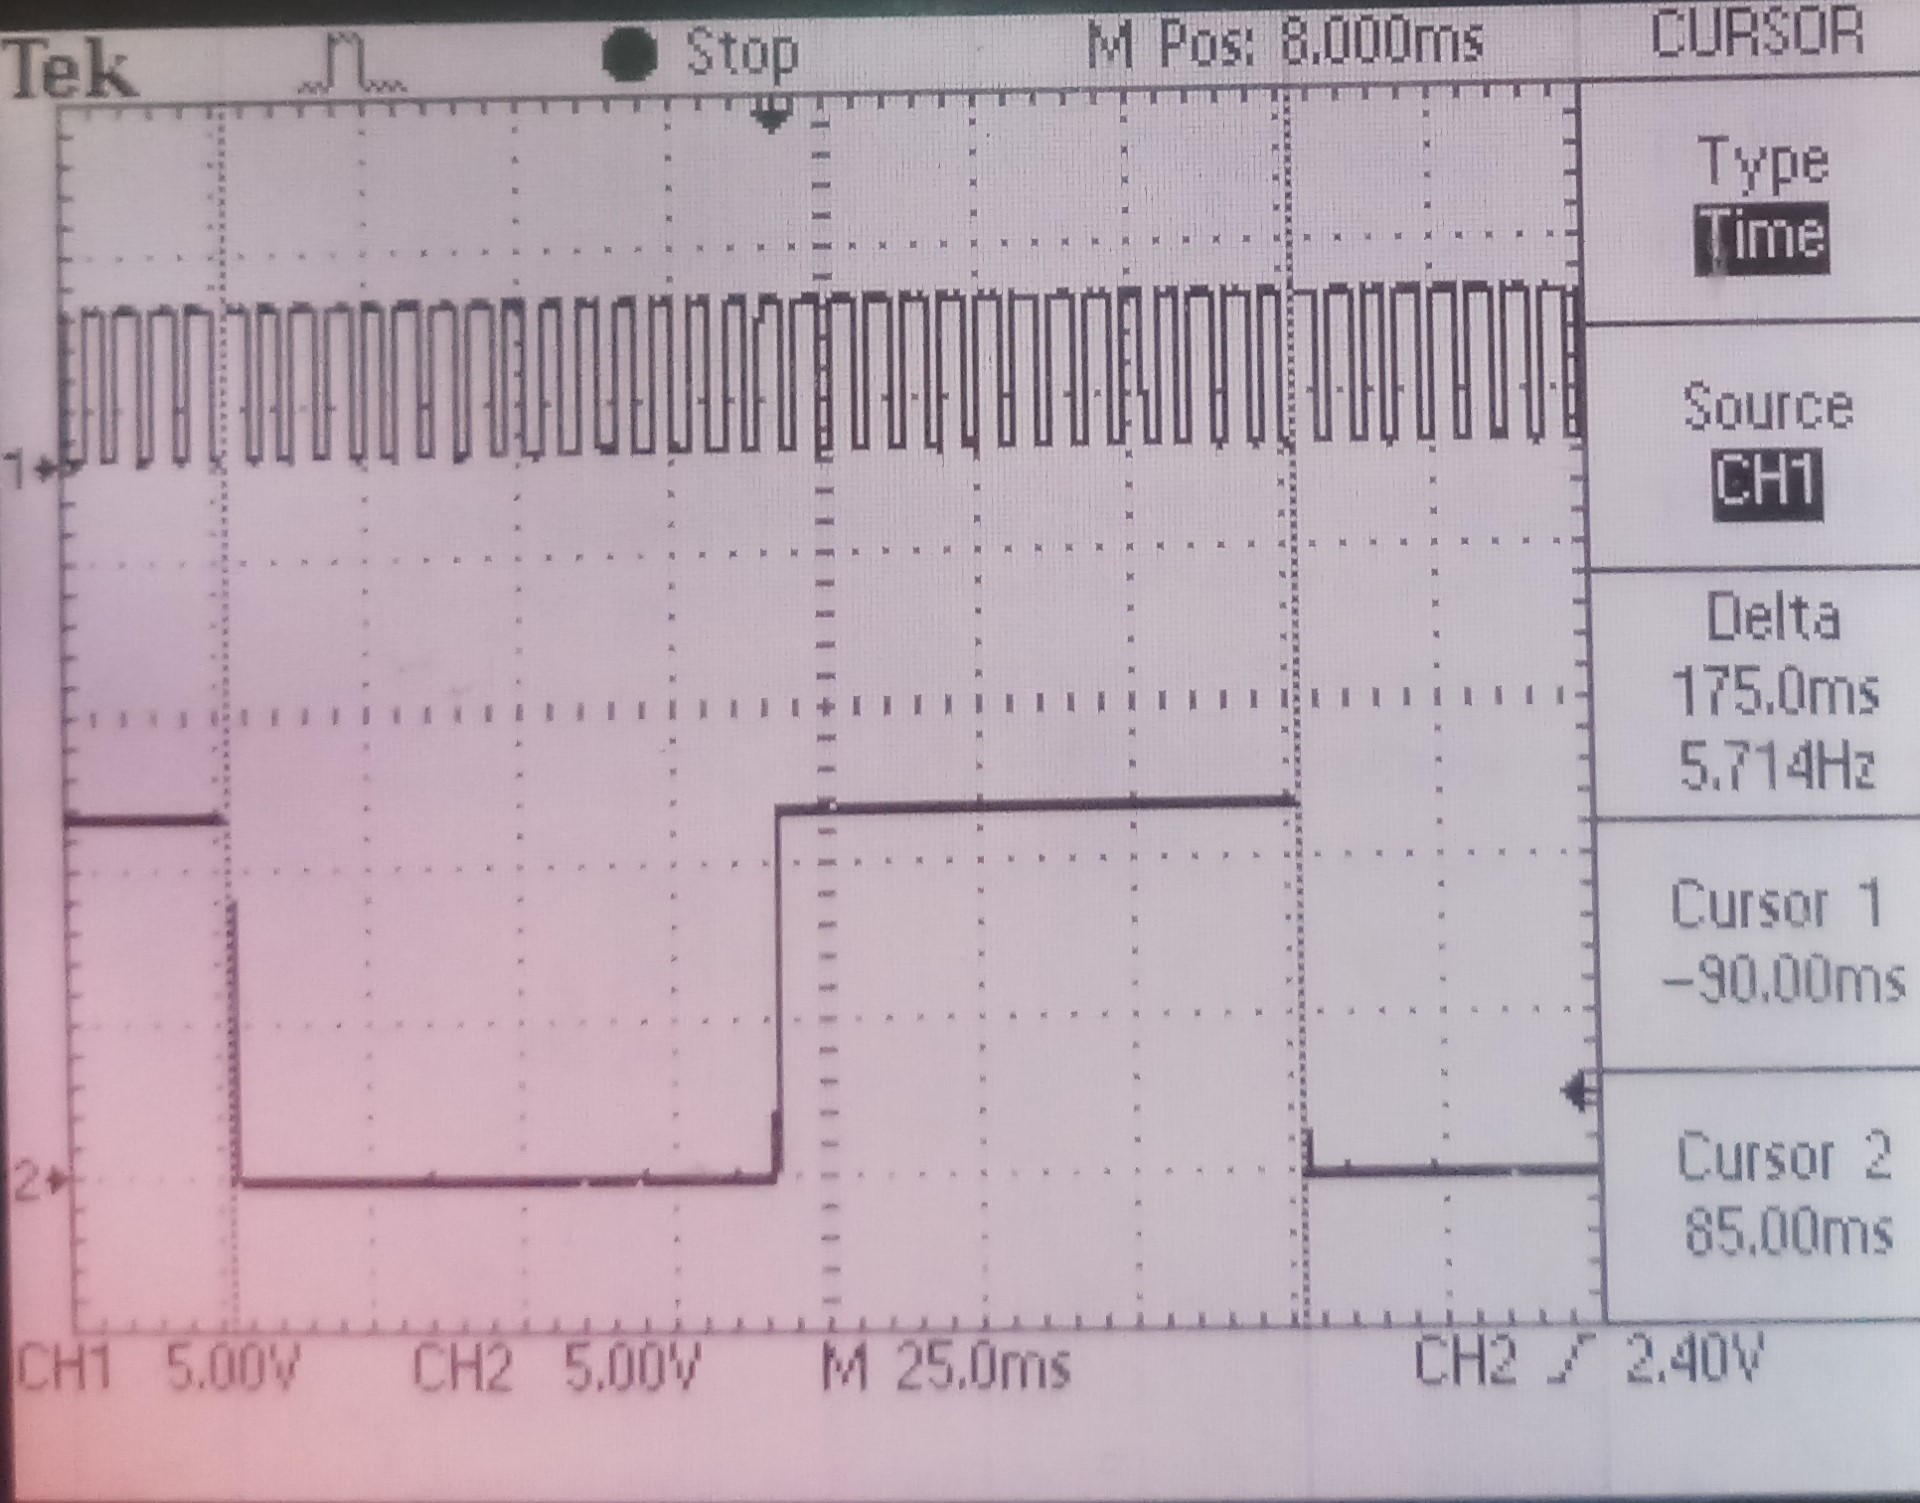
\includegraphics[width = \linewidth, trim = {0 0 0 0}, clip]{HES9V.jpg}
		\caption{\( \nu_{HES} \)}
	\end{subfigure}
	\begin{subfigure}[b]{0.5\linewidth}						
		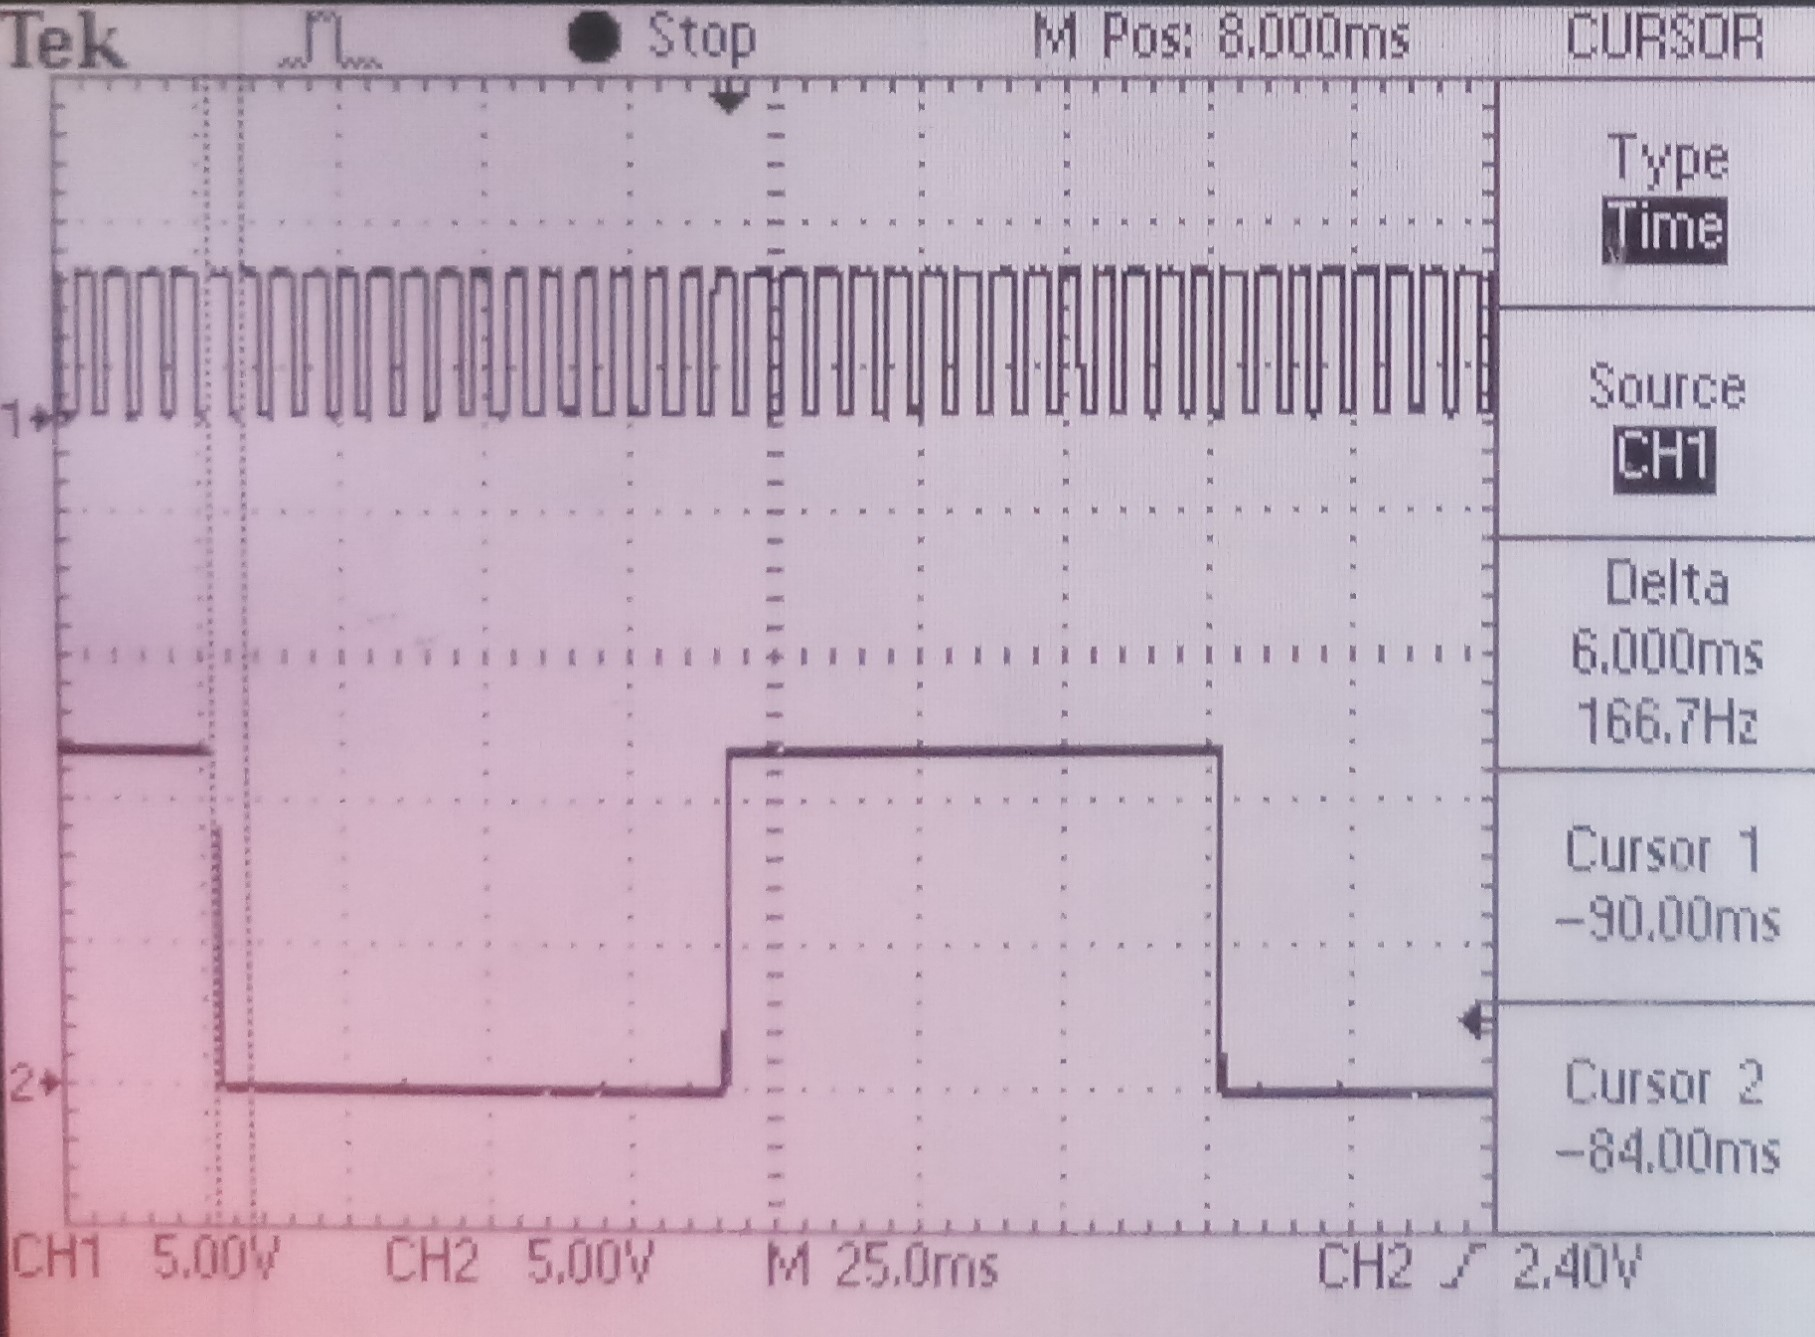
\includegraphics[width = \linewidth, trim = {0 0 0 0}, clip]{IR9V.jpg}
		\caption{\( \nu_{IR} \)}
	\end{subfigure}
	\caption{Oscillator snapshots for 9V}
\end{figure}


Answering the questions in the handouts, the frequency of output of the IR pair sensor was expected to be 30 times the frequency of ouput of the Hall-effect sensor since there were 30 spokes on the wheel attached to the DC motor. The output received in the lab matched this expectation.\\
Moreover, the frequency measured by the Hall-effect sensor (\(f_{HES}\)) represents the frequency of the motor. Hence the speed of the motor is given by the: \[ u_{MOTOR} = f_{HES}\ Hz = 60*f_{HES}\ RPM \]
The fastest speed measurable using the Hall-effect sensor will depend on the slew rate of the operational amplifier used in LM311 and also on the maximum possible frequency of the Digital Storage Oscilloscope (DSO). The fastest speed measurable using the IR pair sensor will also depend on the pick-up of the sensor.

\section{Simulation results}

The code for the comparator circuit which uses IC LM311 is given below:
\begin{verbatim}
Comparator using LM311

.include lm311.txt
x1 1 2 3 4 5 6 LM311
vdd 3 0 12v
vss 4 0 0v
vdummy 6 0 0v
r1 3 5 18k
vref 2 0 2v
vin 1 0 sin(5 5 1k 0 0)

.tran 0.02ms 5ms

.control
run

plot v(1) v(2) v(5)

set hcopydevtype = postscript
set hcopypscolor = 1
hardcopy Comparator_Exercise v(1) v(5)

.endc
.end
\end{verbatim}

\begin{figure}[H]
	\centering
	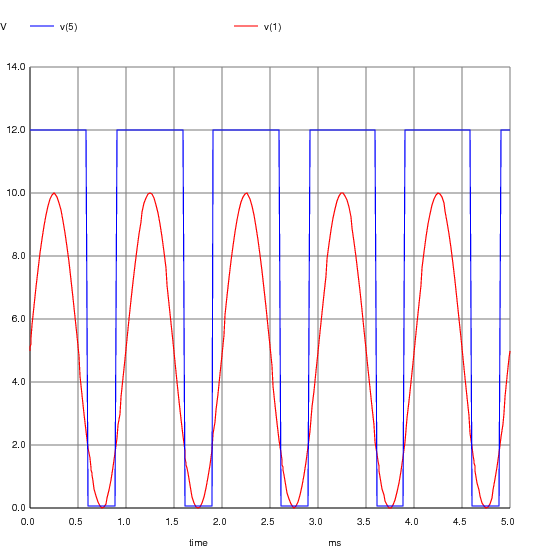
\includegraphics[width = 0.75\linewidth, trim = {0 0 0 0}, clip]{Comparator_Exercise.png}
	\caption{Simulation of the Comparator Circuit}
\end{figure}

\section{Inference}

\subsection{Part 1}

From this part, we infer that the voltage induced due to a magnetic flux causing lateral voltage in a conductor (Hall effect) in the Hall-effect sensor is inversely proportional to the distance of the source of the magnetic flux, which is the Neodymium magnet in this case. This inverse proportionality is non-linear in nature.

\subsection{Part 2}

From this part, we infer that the voltage induced in the Hall-effect sensor is directly proportional to the current passing through the solenoid. The current causes a linearly proportional magnetic field which in turns causes a linearly proportional magnetic flux through the sensor.

\subsection{Part 3}

One can notice from this part that the IR pair sensor measures the product of the number of spokes and the frequency of the motor since it gives a cycle of HIGH and LOW for each spoke. On the other hand, the Hall-effect sensor combined with the comparator circuit measures the frequency of the magnet passing by the sensor face. This frequency is equal to the rotational frequency of the DC motor since the magnet is stationary with respect to the motor and there is a single magnet in the system.

\section{Learning objectives}

The learning objective, with respect to the experiment, was to introduce us to the concept of Lorentz force based sensors and to help integrate several circuits for a common goal. For example, in part 2, we integrated the Hall-effect sensor, a non-inverting amplifier, an offset-removal circuit and a solenoid circuit for the experiment.\\
Looking at the bigger picture, the experiment was a motivation to learn about how electrical systems operate. The experiment gave a real life application of electronic devices and circuits via part 3, where we measured the speed of a DC motor.

\section{Quick feedback}

The Teaching Assistants and Research Assistants are extremely helpful. The experiment has also been well-framed and the experience was well-executed thanks to the whole teaching staff and others relevant.\\
However though I performed the required, I did not see the point in using \textit{several} voltages in the tird part of the experiment since the experiment was to deal with \textit{how} the Hall-effect sensor measures the frequency of the DC motor via the Neodymium magnet.

\subsection{What about this experiment did you find helpful?}
I felt that the whole experiment was useful. Also, on being motivated by one of the videos of Texas Instruments related to Hall-effect sensor, I may design and build a door sensor circuit based on the same sensor.
\subsection{What about this experiment is still unclear?}
I do not find anything unclear from the experiment.

\end{document}